\documentclass[
	% -- opções da classe memoir --
	article,			% indica que é um artigo acadêmico
	11pt,				% tamanho da fonte
	oneside,			% para impressão apenas no recto. Oposto a twoside
	a4paper,			% tamanho do papel. 
	twocolumn,
	% -- opções da classe abntex2 --
	%chapter=TITLE,		% títulos de capítulos convertidos em letras maiúsculas
	%section=TITLE,		% títulos de seções convertidos em letras maiúsculas
	%subsection=TITLE,	% títulos de subseções convertidos em letras maiúsculas
	%subsubsection=TITLE % títulos de subsubseções convertidos em letras maiúsculas
	% -- opções do pacote babel --
	english,			% idioma adicional para hifenização
	brazil,				% o último idioma é o principal do documento
	sumario=tradicional
	]{abntex2}

\usepackage{cmap}	
\usepackage{lmodern}	
\usepackage[T1]{fontenc}	
\usepackage[utf8]{inputenc}		
\usepackage{lastpage}		
\usepackage{color}	
\usepackage{graphicx}	
\usepackage{units}
\usepackage[brazilian,hyperpageref]{backref}
\usepackage[num]{abntex2cite}
\usepackage{bold-extra}
\usepackage{eso-pic}
\usepackage{indentfirst, microtype}		
\usepackage{caption,subcaption,float, dcolumn}
\usepackage{amsfonts,amsmath,amssymb}
\usepackage{enumerate}
\usepackage{titlesec}

\usepackage{multirow}


\usepackage{algpseudocode}
\usepackage{algorithm}

\floatname{algorithm}{Algoritmo}
\renewcommand{\algorithmicrequire}{\textbf{Input:}}
\renewcommand{\algorithmicensure}{\textbf{Output:}}

\usepackage{svg}

\usepackage{listings}
\usepackage[newfloat]{minted}
% \usemintedstyle{friendly}
\citebrackets[]

\usemintedstyle{friendly}
\newenvironment{code}{\captionsetup{type=listing}}{}
\SetupFloatingEnvironment{listing}{name=Código}

\newcommand{\algorithmautorefname}{Algoritmo}
\renewcommand{\backrefpagesname}{Citado na(s) página(s):~}
\renewcommand{\backref}{}
\renewcommand*{\backrefalt}[4]{
	\ifcase #1 %
		Nenhuma citação no texto.%
	\or
		Citado na página #2.%
	\else
		Citado #1 vezes nas páginas #2.%
	\fi}%
% ---

\definecolor{blue}{rgb}{0, .226, .437}
\makeatletter
\hypersetup{
pdftitle={Circuito digital CMOS para controle do fator de qualidade de um filtro passa-banda ativo sintonizável}, 
		pdfauthor={Alef de Oliveira Santos},
    	pdfsubject={TCC2},
	    pdfcreator={LaTeX with abnTeX2},
        pdfkeywords={Fator Q. Controle digital. Métodos numéricos. RTL. Verilog.},
		colorlinks=true,       		% false: boxed links; true: colored links
    	linkcolor=blue,          	% color of internal links
    	citecolor=blue,        		% color of links to bibliography
    	filecolor=magenta,      		% color of file links
		urlcolor=blue,
		bookmarksdepth=4
}
\makeatother
\setlength{\parindent}{1.3cm}
\setlength{\parskip}{0.2cm}  
\makeindex

\renewcommand{\listalgorithmname}{Lista de algoritmos}

\titleformat{\chapter}     {\normalfont\normalsize\bfseries}{\thechapter}     				 {1em}{}
\titleformat{\section}     {\normalfont\normalsize}{\thechapter.\thesection}     			 {1em}{}
\titleformat{\subsection}  {\normalfont\normalsize}{\thechapter.\thesection.\thesubsection}  {1em}{}


\setlrmarginsandblock{1.5cm}{1.5cm}{*}
\setulmarginsandblock{1.5cm}{2.5cm}{*}
\checkandfixthelayout



\usepackage{config/customizacoes}

\instituicao{
  Universidade Federal de Itajubá -- UNIFEI
  \par
  \textit{Campus} Theodomiro Carneiro Santiago
  \par
  Instituto de ciências tecnológicas -- ICT
}

\curso{Engenharia da computação}

% Título e subtítulo
\titulo{Circuito digital de controle do fator de qualidade de um filtro passa-banda ativo sintonizável}


% Participantes
\autor{Alef de Oliveira Santos}
\orientador{Dr. Dean Bicudo Karolak}
\coorientador{Dr. Paulo Márcio Moreira E Silva}

\local{Itabira, MG}
\data{\today}


\tipotrabalho{Trabalho de Conclusão de Curso - TCC}

\preambulo{Monografia submetida ao curso de graduação em \imprimircurso\ da Universidade federal de Itajubá, como requisito parcial para obtenção do título de Bacharel em \imprimircurso.}


% Dados para a ficha catalográfica
\palavraChaveUm{Palavra-chave01}
\palavraChaveDois{Palavra-chave02}

\cdu{02:141:005.6} % nao sei qq eh

% Dados da aprovação do trabalho
\dataDaAprovacao{01 de junho de 2013}
\membroConvidadoUm{Dr. Rodrigo Aparecido da Silva Braga}
\membroConvidadoDois{Dr. Diogo Leonardo da Silva}




\begin{document}



\frenchspacing 
\imprimircapa
\imprimirfolhaderosto*

% \begin{fichacatalografica}
	\vspace*{\fill}					% Posição vertical
	\hrule							% Linha horizontal
	\begin{center}					% Minipage Centralizado
	\begin{minipage}[c]{12.5cm}		% Largura
	
	\imprimirautor
	
	\hspace{0.5cm} \imprimirtitulo  / \imprimirautor. --
	\imprimirlocal, \imprimirdata-
	
	\hspace{0.5cm} \pageref{LastPage} p. : il. (algumas color.) ; 30 cm.\\
	
	\hspace{0.5cm} \imprimirorientadorRotulo~\imprimirorientador\\
	
	\hspace{0.5cm}
	\parbox[t]{\textwidth}{\imprimirtipotrabalho~--~\imprimirinstituicao,
	\imprimirdata.}\\
	
	\hspace{0.5cm}
		1. \imprimirpalavrachaveum.
		2. \imprimirpalavrachavedois.
		I. \imprimirorientador.
		II. \imprimircoorientador
		III. \imprimirinstituicao
        IV. Instituto de ciências tecnológicas
		V. \imprimirtitulo\\ 			
	
	\hspace{8.75cm} CDU \nomecdu\\
	
	\end{minipage}
	\end{center}
	\hrule
\end{fichacatalografica}


% \begin{errata}
Elemento opcional da \citeonline[4.2.1.2]{NBR14724:2011}. \textbf{Caso não 
deseje uma errata, deixar todo este arquivo em branco}. Exemplo:

\vspace{\onelineskip}

FERRIGNO, C. R. A. \textbf{Tratamento de neoplasias ósseas apendiculares com
reimplantação de enxerto ósseo autólogo autoclavado associado ao plasma
rico em plaquetas}: estudo crítico na cirurgia de preservação de membro em
cães. 2011. 128 f. Tese (Livre-Docência) - Faculdade de Medicina Veterinária e
Zootecnia, Universidade de São Paulo, São Paulo, 2011.

\begin{table}[htb]
\center
\footnotesize
\begin{tabular}{|p{1.4cm}|p{1cm}|p{3cm}|p{3cm}|}
  \hline
   \textbf{Folha} & \textbf{Linha}  & \textbf{Onde se lê}  & \textbf{Leia-se}  \\
    \hline
    1 & 10 & auto-conclavo & autoconclavo\\
   \hline
\end{tabular}
\end{table}

\end{errata}


\begin{folhadeaprovacao}

  \begin{center}
    {\ABNTEXchapterfont\large\imprimirautor}

    \vspace*{\fill}\vspace*{\fill}
    {\ABNTEXchapterfont\bfseries\Large\imprimirtitulo}
    \vspace*{\fill}
    
    \hspace{.45\textwidth}
    \begin{minipage}{.5\textwidth}
        \imprimirpreambulo
    \end{minipage}%
    \vspace*{\fill}
   \end{center}
    
   Trabalho \verb|_______________|. \imprimirlocal, \imprimirdatadaaprovacao:

   \assinatura{\textbf{\imprimirorientador} \\ Orientador}
   \assinatura{\textbf{\imprimircoorientador} \\ Co-orientador}
   \assinatura{\textbf{\imprimirmembroconvidadoum} \\ Membro da banca}
   \assinatura{\textbf{\imprimirmembroconvidadodois} \\ Membro da banca}
      
   \begin{center}
    \vspace*{0.5cm}
    {\large\imprimirlocal}
    \par
    {\large\imprimirdata}
    \vspace*{1cm}
  \end{center}
  
\end{folhadeaprovacao}

\begin{dedicatoria}
    \vspace*{\fill}
    \flushright
    \noindent
    % \begin{minipage}[0.3]
    \textit{Dedico este trabalho àqueles que lutam \\ para popularizar a ciência.}
    % \end{minipage}
\end{dedicatoria}

\begin{agradecimentos}

Agradeço ao professor Rodrigo por despertar em mim o interesse sobre o tema de microeletrônica. Aos professores Dean e Paulo pela orientação e paciência em ensinar nestes anos de pesquisa. Ao Maderson e à Cristina pelo suporte e confiança. À Larissa pela lista de inúmeras contribuições, particularmente, fora deste trabalho. 


\end{agradecimentos}

% \begin{epigrafe}
    \vspace*{\fill}
	\begin{flushright}
		\textbf{A epígrafe é opcional. Caso não deseje uma, deixe todo
		este arquivo em branco}.

		\textit{``Não vos amoldeis às estruturas deste mundo, \\
		mas transformai-vos pela renovação da mente, \\
		a fim de distinguir qual é a vontade de Deus: \\
		o que é bom, o que Lhe é agradável, o que é perfeito.\\
		(Bíblia Sagrada, Romanos 12, 2)}
	\end{flushright}
\end{epigrafe}


\begin{resumo}
 % O resumo deve ressaltar o objetivo, o método, os resultados e as conclusões 
 % do documento. A ordem e a extensão
 % destes itens dependem do tipo de resumo (informativo ou indicativo) e do
 % tratamento que cada item recebe no documento original. O resumo deve ser
 % precedido da referência do documento, com exceção do resumo inserido no
 % próprio documento. (\ldots) As palavras-chave devem figurar logo abaixo do
 % resumo, antecedidas da expressão Palavras-chave:, separadas entre si por
 % ponto e finalizadas também por ponto. O texto pode conter no mínimo 150 e 
 % no máximo 500 palavras, é aconselhável que sejam utilizadas 200 palavras. 
 % E não se separa o texto do resumo em parágrafos.

 O controle do fator de qualidade ($Q$) em um filtro passa banda é uma maneira direta de controlar a seletividade deste filtro, e utilizando um circuito ativo é possível controlá-lo. Para controlar o $Q$ de um sistema ressonante com um circuito digital utiliza-se neste trabalho técnicas de computação numérica para aproximação de funções não-lineares, uma vez que os parâmetros do filtro \textit{on-chip} não são manipuláveis além da corrente que controla o $Q$. Assim, o objetivo deste trabalho é projetar um circuito digital sintetizável capaz de: receber como entrada o $Q$  desejado e medido de um filtro passa banda e controlar digitalmente esse valor de $Q$ do filtro. Além disso, três diferentes métodos numéricos de controle serão estudados e implementados para comparação e escolha do melhor método de convergência.
 
 % Desta forma, objetivo deste trabalho é documentar o projeto de um circuito digital capaz de receber como entrada um $Q$ desejado e controlar o fator de qualidade de um filtro ativo por meio da corrente injetada em um oscilador LC, utilizando e comparando 3 diferentes métodos numéricos para controle deste fator $Q$.

 \vspace{\onelineskip}
    
 \noindent
 \textbf{Palavras-chave}: Fator Q. Controle digital. Métodos numéricos. RTL. Verilog.
\end{resumo}

\begin{resumo}[Abstract]
 \begin{otherlanguage*}{english}
     Tuning the quality factor ($Q$) in a bandpass filter is a direct way to control the filter's selectivity, and this goal can be achieved by using an active circuit. In order to control the $Q$ of a resonant system with a digital circuit, this work uses numerical computing techniques to approximate non-linear functions, since the parameters of the \textit{on-chip} filter are not manipulable beyond the current that controls the $Q$. Thus, the aim of this work is to design a synthesizable digital circuit capable of: receiving as input the desired and measured $Q$ of a bandpass filter and digitally and digitally adjust its bias current to achieve a $Q$ value close to the desired one. Therefore, the system architecture is basically composed by digital circuits to determine the measured filter $Q$ value, to compare it with the desired value and tune it as close as possible to the desired value. Regarding the Q adjustment block, three different numerical control methods are studied and implemented in order to compare and choose the best convergence method.

   \vspace{\onelineskip}
 
   \noindent 
   \textbf{Key-words}: Q factor. Digital control. Numerical methods. RTL. Verilog.
 \end{otherlanguage*}
\end{resumo}


% elementos de enumerações
% Lista de figuras e tabelas
\pdfbookmark[0]{\listfigurename}{lof}
\listoffigures*
\cleardoublepage
\pdfbookmark[0]{\listtablename}{lot}
\listoftables*
\cleardoublepage


\listofalgorithms*
\addtocontents{loa}{\def\string\figurename{Algoritmo}}
\cleardoublepage

% abreviaturas e siglas

\begin{siglas}
  \item [A/D  ] Analógico para Digital (conversão) 
  \item [CI   ] Circuito Integrado
  \item [CC   ] \textit{Clock Cycle}
  \item [D/A  ] Digital para Analógico (conversão) 
  \item [DAC  ] \textit{Digital-to-analog converter}
  \item [DFT  ] \textit{Design for testability}
  \item [DUT  ] \textit{Device Under Test}
  \item [EDA  ] \textit{Electronic design automation}
  \item [GDSII] \textit{Graphic Design System} II
  \item [HDL  ] \textit{Hardware Description Language}
  \item [ITC  ] \textit{Iterations-to-converge}
  \item [RF   ] Rádio-Frequência/\textit{Radio-Frequency}
  \item [STA  ] \textit{Static timing analysis}
  \item [TB   ] \textit{Testbench(es)}
  \item [UVM  ] \textit{Universal Verification Methodology}
  % \item [$I_{REF}$] Corrente de referência
  % \item [$I_{REF}|_{Setup}$]Corrente de referência para configuração
\end{siglas}


% simbolos

\begin{simbolos}
  \item[$\alpha$] Alfa
  \item[$ \Delta $] Delta
  \item[$\beta$] Beta
  \item[$\varepsilon$] Épsilon (erro)
  \item[$Q$] Fator de Qualidade 
  \item[$\hat{Q}$] Fator de qualidade aproximado por algoritmo
  \item[$Q_d$] Fator de qualidade desejado
  \item[$Q_m$] Fator de qualidade medido
  \item[$\gamma$] Gama
  \item[$\gets$] Atribuição em algoritmos (recebe)
  \item[$\vee$] Disjunção
  \item[$\wedge$] Conjunção
  % \item[$ \Lambda $] Lambda
  % \item[$ \zeta $] Letra grega minúscula zeta
  % \item[$ \in $] Pertence
\end{simbolos}




% Sumário
\pdfbookmark[0]{\contentsname}{toc}
\tableofcontents*
\cleardoublepage

% \input{config/indiceAutomatico}

\textual

\part{Introdução}

\chapter{Introdução}

% o que é o quê e por quê ele é importante?
% como medir o Q
% [ENFASE] como controlar o Q 
% 

Este trabalho trata de um sistema eletrônico que recebe e controla o fator de qualidade ($Q$) de um circuito eletrônico ressonante. O circuito proposto utiliza-se de técnicas de computação numérica para controlar o fator de qualidade através de uma corrente de referência injetada no sistema ressonante. Neste trabalho serão realizados circuitos digitais periféricos para a determinação do valor de $Q$ medido de um filtro passa banda ativo, bem como, um circuito digital para controle e aproximação do $Q$ desejado. Em relação ao controle e aproximação de Q, serão comparados os métodos numéricos da Bisseção, Secantes e Secantes com seleção de intervalo implementados. O sistema digital é projetado e implementado em Verilog tendo em mente a posterior fabricação em silício. Para efeitos de estudo e desenvolvimento, este projeto em ASIC utiliza uma tecnologia GPDK de 45nm.

% Neste trabalho serão realizados circuitos digitais periféricos para a determinação do valor de Q medido de um filtro passa banda ativo, bem como, um circuito digital para controle e aproximação do Q desejado. Em relação ao controle e aproximação de Q, serão comparados...

\section{Contexto e justificativa}

A caracterização fator de qualidade ($Q$) é um ponto de partida para projetos de circuitos integrados de rádio-frequência de alto desempenho \cite{what-is-q-takashi}. Ele está relacionado com a largura de banda de um filtro passa-banda e, por vezes, os projetistas de filtros necessitam de uma largura de banda estreita (isto é, alto $Q$) e em outras, uma banda maior (baixo $Q$) como ilustra a \autoref{f-banda-q}:

\begin{figure}[H]
    \centering
    \caption{$Q$ \textit{versus} largura de banda}
    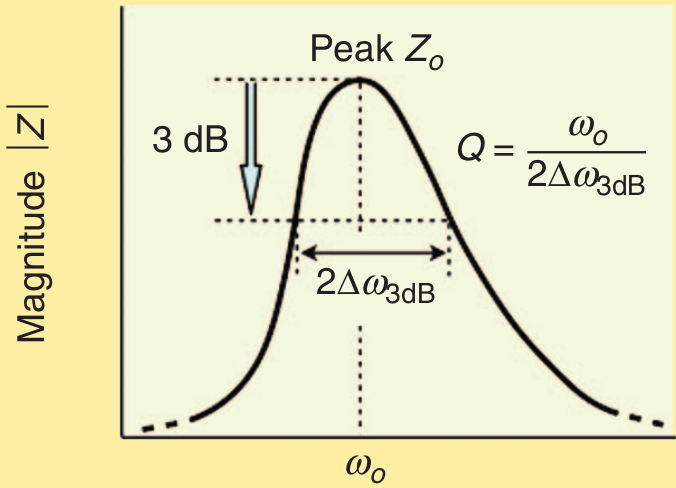
\includegraphics[width=.5\textwidth]{fig/q-band.png}
    \legend{Fonte: \cite{what-is-q-takashi}}
    \label{f-banda-q}
\end{figure}

% Da teoria de sistemas de controles dinâmicos, mudar a resposta em frequência do projeto de filtros,

% No trabalho de \autoref{z-matching}

Ainda de acordo com \citeauthor{what-is-q-takashi}, o fator $Q$ também está relacionado com o teorema da máxima transferência de potência em circuitos de RF. Para entregar o máximo de potência de uma fonte para uma carga através de uma rede, um circuito de casamento de impedâncias é usado para alcançar a maior transferência de potência. A \autoref{f-eff-q} ilustra como o $Q$ interfere na eficiência de um circuito:


\begin{figure}[H]
    \centering
    \caption{$Q$ \textit{versus} eficiência}
    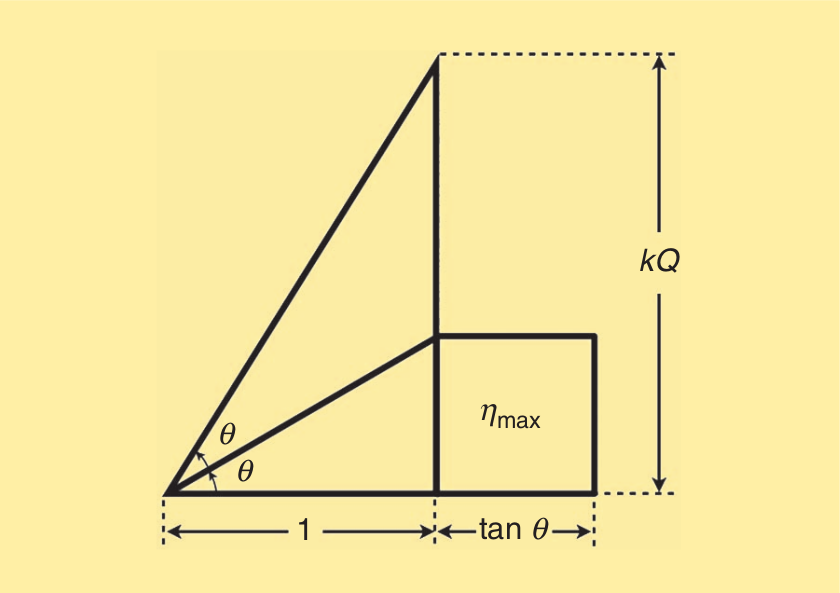
\includegraphics[width=.5\textwidth]{fig/q-eff.png}
    \legend{Fonte: \cite{what-is-q-takashi}}
    \label{f-eff-q}
\end{figure}


Num circuito com uma carga estática, basta calcular um $Q$ que realize o casamento de impedâncias para a maior transferência de potência. Num circuito onde a carga é variável, um $Q$ fixo não fornece o casamento de impedâncias necessário para a máxima transferência de potência em todos os cenários de carregamento, assim reduzindo a eficiência do circuito. 

De fato \citeauthor{z-match-q} retomam em seu trabalho as proposições de \citeauthor{what-is-q-takashi} e projetam uma rede de casamentos de impedância baseada no fator de qualidade, onde o mesmo é ajustado a fim de casar impedâncias de rede com uma carga variável. \citeauthor{z-match-q-2} realiza um trabalho com a mesma ideia de controlar o $Q$ usando outras técnicas para selecionar o valor ótimo.


% Em sistemas sensores microeletromecânicos (MeMS) o fator de qualidade está atrelado à resolução e à estabilidade em frequência. Um baixo $Q$ resulta em baixa resolução e alta estabilidade em  altas frequências, enquanto um $Q$ alto é o inverso dessas características  \cite{mems-two-inductors}. 

% No trabalho de \citeauthor{mems-two-inductors} foram utilizados dois indutores, sendo um com baixo fator de qualidade e outro com alto, para combiná-los em série e obter um $Q$ intermediário com sensibilidade e estabilidade em frequência suficientes para a aplicação proposta. Sob essa perspectiva, o trabalho aqui desenvolvido seria um adicional relevante pois seria necessário projetar no trabalho de  \citeauthor{mems-two-inductors} apenas um indutor com alto fator de qualidade e controlar o $Q$ da mesma forma proposta neste trabalho. Isso se torna particularmente ainda mais relevante uma vez que o oscilador usado no trabalho de \citeauthor{mems-two-inductors} é similar ao oscilador LC de par cruzado usado neste trabalho, vide \autoref{f-osciladores}.

% % \begin{figure}[H]
% %     \centering
% %     \caption{\textcolor{red}{Comparação entre osciladores usados}}
% %     \begin{subfigure}[H]{.49\textwidth}
% %         \centering
% %         \caption{Oscilador usado neste trabalho}
% %         % 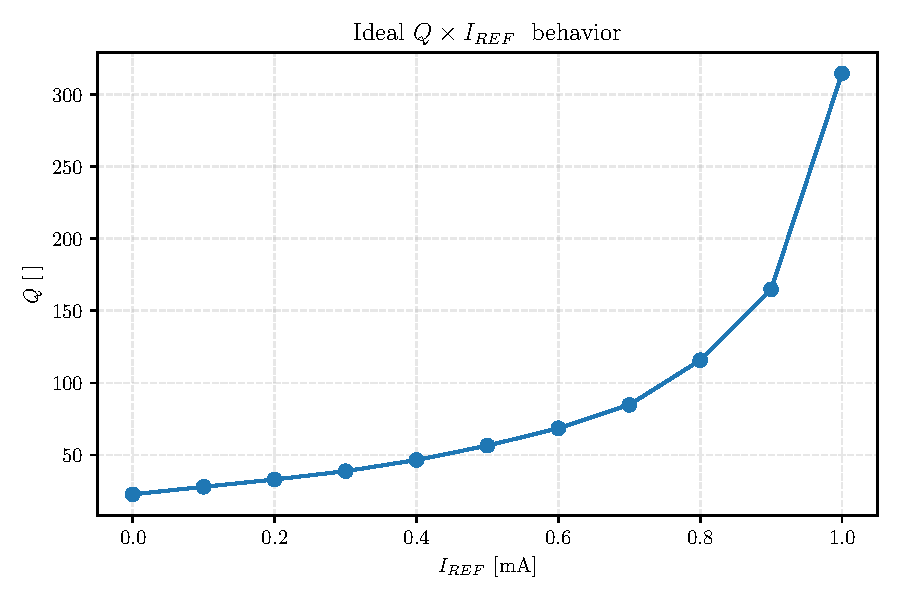
\includegraphics{fig/q-no-drop.pdf}
% %         \legend{Fonte: Adaptado de \cite{tese-pmms}}
% %         % \label{}
% %     \end{subfigure}
% %     \hfil
% %     \begin{subfigure}[H]{.49\textwidth}
% %         \centering
% %         \caption{Oscilador do trabalho de \citeauthor{mems-two-inductors}}
% %         % 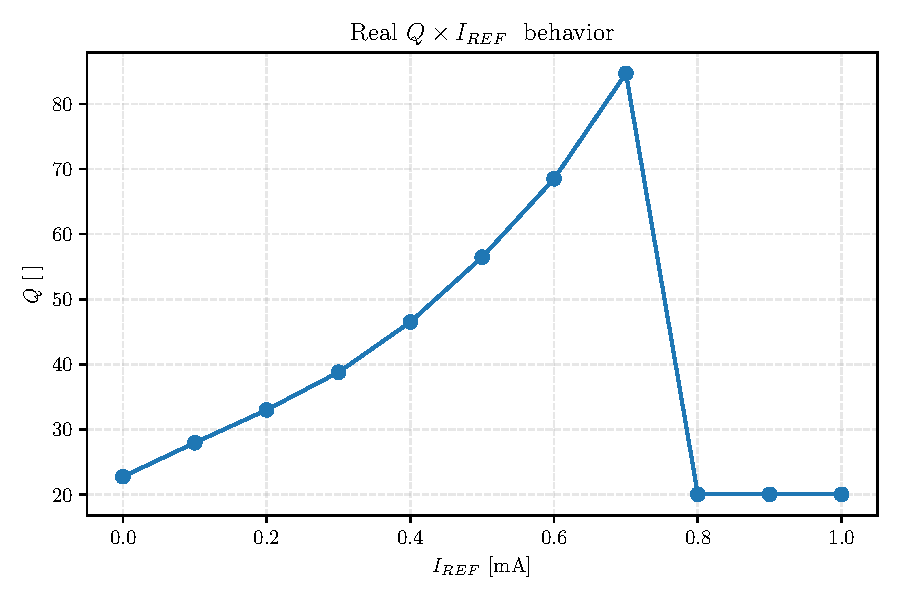
\includegraphics{fig/q-with-drop.pdf}
% %         \legend{Fonte: \cite{mems-two-inductors}}
% %         % \label{}
% %     \end{subfigure}
% %     \hfil
% %     \label{f-osciladores}
% % \end{figure}

% Vistas as similaridades dos osciladores usados, adaptar o circuito de \citeauthor{mems-two-inductors} para o trabalho em questão, usando um único indutor integrado de alto fator de qualidade
% pode ser uma opção viável. De fato projetar um único indutor de alto $Q$ não é tarefa trivial mas a indústria de RF têm avançado e é possível ver indutores com fatores elevados de qualidade, assim como desenvolvidos nos trabalhos de \citeonline{high-q-1} e \citeonline{high-q-2}.


Desta forma, fica evidente a necessidade de controlar o $Q$ de um circuito eletrônico, tanto no contexto deste trabalho quanto em outros trabalhos com pouca similaridade, mas com a mesma necessidade de $Q$ controlável/variável. 


Em relação às diferentes implementações de circuitos eletrônicos para controle do $Q$, pode-se distingui-los em dois grupos, os circuitos analógicos e os digitais. Os circuitos analógicos têm a vantagem de ser mais simples, mais rápidos, como apresentado em \cite{z-match-q-2}. Entretanto, eles não apresentam a mesma versatilidade e configurabilidade proposta por um sistema digital. Já os circuitos digitais, além de mais versáteis, apresentam uma implementação física mais simples com o uso de \textit{standard-cells} para a construção de \textit{layouts}, sendo inclusive, altamente assistidas por ferramentas de EDA pela característica programática. Em conjunto com a maior versatilidade, o circuito digital poderia ser estendido em aplicações onde o controle do $Q$ deve ter alta precisão, uma vez que o circuito digital pode ser replicado com maior confiabilidade, portabilidade e reprodutibilidade. \\



% \begin{itemize}
%     \item \textit{Layout}: O processo de layout digital utilizando-se de \textit{standard cells} é mais rápido e simples de se fazer comparado ao \textit{layout} analógico \cite{the-art-of-layout}
% \end{itemize}


Dessa forma, julga-se pertinente projetar este circuito eletrônico digital capaz de controlar o $Q$, para que seja possível obter circuitos mais versáteis e com aplicações mais amplas com menor complexidade em projeto analógico, além de promover inovação no desenvolvimento de circuitos para computação numérica.





% \section{Trabalhos similares}



\chapter{Objetivos}\label{ch-obj}

Os objetivos principais deste trabalho para o TCC1 são, principalmente o fluxo de front-end, compreendido por:

\begin{enumerate}
    \item Projetar a arquitetura capaz de controlar o fator de qualidade do circuito;
    % \item Adaptar métodos numéricos e prototipá-los em alto nível
    \item Codificar os blocos do sistema projetado em Verilog;
    \item Comparar o desempenho dos métodos de controle prototipados \textit{standalone};
    \item Validar a funcionalidade blocos projetados através de \textit{testbenches} em Verilog/SystemVerilog.
\end{enumerate}


Após finalizado o fluxo de front-end, seleciona-se o método de convergência com melhor desempenho com relação à todo o sistema e inicia-se o processo de verificação do sistema completo seguido do fluxo de back-end no TCC2, compreendido por:

\begin{enumerate}
    \item Integrar e coordenar a operação dos blocos como um sistema completo;
    \item Realizar a síntese lógica em RTL;
    \item Simular o circuito sintetizado em RTL e checar a equivalência lógica;
    \item Realizar etapas de posicionamento e roteamento;
    \item Analisar o consumo;
    \item Analisar desempenho do sistema por temporização estática (STA);
    \item Construir layout.
\end{enumerate}


\part{Desenvolvimento}

\chapter{Referencial teórico}\label{ch-referencial}

\section{Interface com o sistema completo e arquitetura simplificada}\label{sec-interface}

Antes de descrever a arquitetura completa desenvolvida neste trabalho, é necessário retomar que o sistema de controle é complementar à um sistema pré-existente composto pelo próprio sistema ressonante\footnote{Baseado em \cite{tese-pmms}} (dentre outras estruturas) e um DAC. Assim sendo, algumas escolhas de arquitetura na verdade são requisitos de integração do projeto e comunicação. A \autoref{f-arq-simplif} ilustra a arquitetura simplificada do sistema completo.

\begin{figure}[H]
    \centering
    \caption{Arquitetura simplificada do sistema completo}
    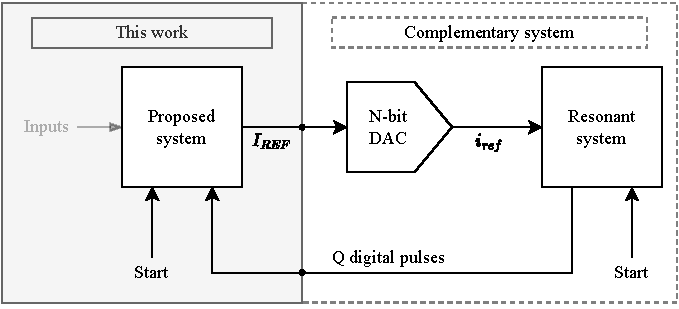
\includegraphics[width=.7\textwidth]{fig/arq-simplif.pdf}
    \label{f-arq-simplif}
\end{figure}

Neste diagrama de blocos há 3 blocos principais. Cada bloco e sua respectiva responsabilidade é:

\begin{enumerate}
    \item \textit{Proposed System}: o próprio sistema digital desenvolvido responsável por controlar o $Q$ fazendo uso dos métodos numéricos descritos na \autoref{sec-metodos-convergencia} -- \nameref{sec-metodos-convergencia}. Também responsável por outras operações relevantes ao ajuste do $Q$, bem como a determinação do valor máximo alcançável de $Q$, recepção do valor de $Q$ dentre outras estruturas. Este bloco é detalhado na \autoref{sec-arquitetura} -- \nameref{sec-arquitetura}.
    \item \textit{Resonant System}: Sistema ressonante controlado por corrente ($i_{ref}$), o qual apresenta um fator de qualidade $Q$ proporcional à corrente de polarização e disponibiliza a medição do $Q$ em um sinal serial \textit{Q digital pulses}.
    \item \textit{Current Control} (N-bit DAC): Conversor D/A que recebe a palavra digital $I_{REF}$ e a converte em um valor analógico $i_{ref}$ que controla o oscilador do sistema ressonante. 
\end{enumerate}


Os blocos supracitados, com suas entradas, saídas, têm suas funcionalidades elencadas na \autoref{tab-arq-simplif}:

\begin{table}[H]
    \centering
    \caption{Sinais, respectivos tipos e funcionalidades por bloco}
    \resizebox{\columnwidth}{!}{%
\begin{tabular}{@{}lp{3cm}lp{13cm}@{}}
\toprule
\textbf{Bloco}           & \textbf{Sinal}            & \textbf{Tipo}              & \textbf{Função referente ao bloco}                                                                    \\ \midrule
\textit{Proposed system} & Start                     & Digital {[}1 bit{]}        & Sinalizar que o oscilador enviará pulsos correspondentes ao valor de $Q$                              \\
\textit{Proposed system} & $I_{REF}$                 & Digital {[}10 bits{]}      & Enviar valor digital de corrente de referência para controlar o $Q$                                   \\
N-bit DAC                & $I_{REF}$                 & Digital {[}10 bits{]}      & Receber valor digital de corrente de referência para conversão D/A\\
N-bit DAC                & $i_{ref}$                 & Analógico                  & Equivalente analógico convertido de $I_{REF}$                                                         \\
\textit{Resonant system} & Start                     & Digital {[}1 bit{]}        & Indicar que o sistema pode injetar a corrente no oscilador LC interno                                 \\
\textit{Resonant system} & \textit{Q digital pulses} & Digital Serial {[}1 bit{]} & Valor de $Q$ medido e convertido em um trem de pulsos                                                 \\ \bottomrule
\end{tabular}%
}
    \label{tab-arq-simplif}
\end{table}

As entradas descritas na \autoref{tab-arq-simplif} e \autoref{f-arq-simplif} são suficientes para a comunicação completa do sistema,  detalhada na \autoref{sec-arquitetura} -- \nameref{sec-arquitetura}. As outras entradas relevantes do sistema proposto (representadas na \autoref{f-arq-simplif} com baixa opacidade) também serão elencadas no detalhamento da arquitetura na seção relativa.


% A medição do fator de qualidade, como elencado na \autoref{tab-arq-simplif}, consiste em receber o trem de pulsos digitais que é proporcional ao valor de $Q$ medido. Um maior número de pulsos indica maior fator de qualidade. A responsabilidade de garantir que a medida seja feita de maneira correta é elencada de forma detalhada seção referente ao detalhamento da arquitetura do sistema. respectiva à medição (\autoref{sec-}



% A medição 

% \textcolor{red}{Exemplificar o processo de medição, esboçar ondas analógicas e o trem de pulsos digtal correspondente. Mostrar o comportamento ideal do Q (sem instabilidade) e o real (com o instabilidade)}

% % A medição do fator de qualidade pode ser feita de formas diferentes segundo as definições propostas na \autoref{sec-fator-q}. Para este trabalho, é usada a medição no domínio do tempo, pois assim pode-se medir o fator de qualidade com o funcionamento natural do circuito oscilador. De fato, esta medição efetiva é implementada pelo sistema pré-existente, mencionado na \autoref{sec-interface}. O sistema faz uma interface A/D de um sinal oscilante no tempo para um trem de pulsos em que a quantidade de pulsos representa o valor aproximado do $Q$ medido, como ilustra a \autoref{f-conversão-simplificada-q}:

% % \begin{figure}[H]
% %     \centering
% %     \caption{Conversão A/D simplificada do $Q$}
% %     % \includegraphics{}
% %     \label{f-conversão-simplificada-q}
% % \end{figure}
 

% \subsubsection{Comportamento ideal}\label{sss-comportamento-ideal-q}

% No comportamento ideal, o $Q$ tende a infinito no momento em que a constante de decaimento desse sistema tende a 0. Assim sendo, idealmente, seria possível alcançar qualquer valor de $Q$ maior que um valor mínimo, como ilustra a \autoref{f-q-ideal}:


% \begin{figure}[H]
%     \centering
%     % \caption{Diagrama de tempo da operação do bloco de seleção de corrente}
%     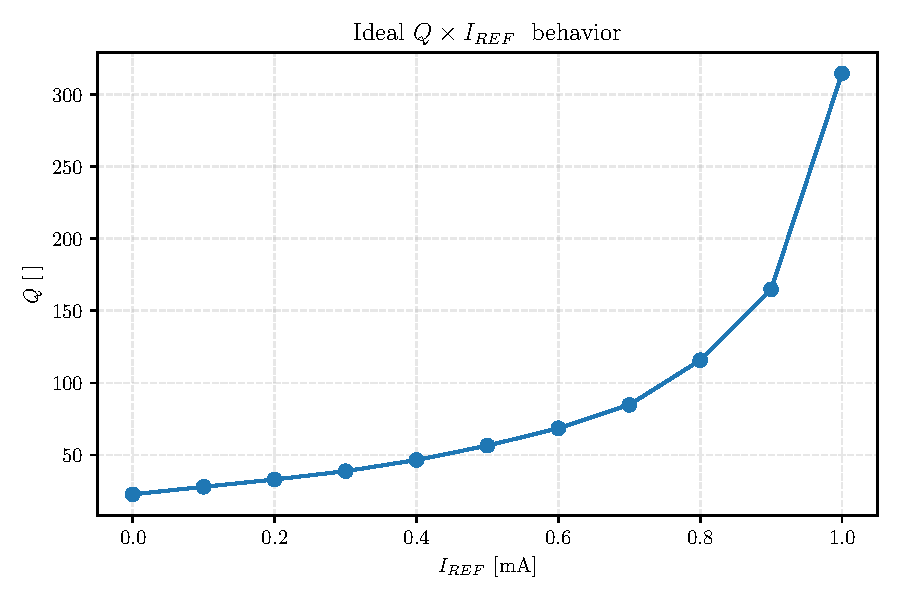
\includegraphics[width=.7\textwidth]{fig/q-no-drop.pdf}
%     \legend{Fonte: o autor}
%     % \label{f-timing-iref-selection}
% \end{figure}




% \subsubsection{Comportamento real}\label{sss-comportamento-real-q}


% No comportamento ideal, o $Q$ tende a infinito no momento em que a constante de decaimento desse sistema tende a 0. No sistema já projetado o $Q$ "infinito" é na verdade um valor muito alto que não consegue ser medido e convertido em trem de pulsos por limitações do sistema de medição. Dessa forma, o sistema ao invés de acusar um fator de qualidade alto, acaba gerando um valor espúrio muito baixo se comparado com o que realmente deveria ser medido, como ilustra a \autoref{f-q-instavel}:

% \begin{figure}[H]
%     \centering
%     % \caption{Diagrama de tempo da operação do bloco de seleção de corrente}
%     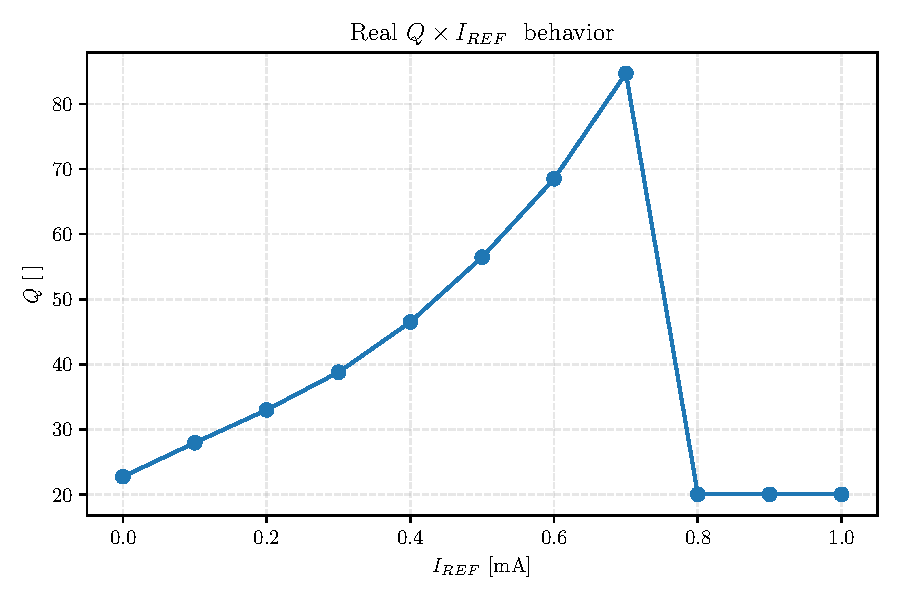
\includegraphics[width=.7\textwidth]{fig/q-with-drop.pdf}
%     \legend{Fonte: o autor}
%     % \label{f-timing-iref-selection}
% \end{figure}


% % Enxerga-se relevante analisar os resultados dos métodos de aproximação para ambos os comportamentos pois pode ser que em outro sistema com um perfil diferente de $I \times Q$ não aconteça a instabilidade. 
% % % \subsection{Controle do fator de qualidade -- $Q \times I_{REF}$}





% % % Em linhas gerais, o funcionamento resumido é composto por 3 etapas:

% % % \begin{enumerate}
% % %     \item É enviado o sinal de \textit{Start} ao bloco de controle e o oscilador, em conjunto com uma corrente inicial para configuração. 
% % %     \item O sistema ressonante converte a oscilação em um trem de pulsos digitais (\textit{Q digital pulses}).
% % %     \item O sistema de controle manipula a corrente até atingir o valor de $Q$ desejado.
% % % \end{enumerate}

% % % .




% \section{Fator de qualidade \textit{versus} corrente de referência -- $Q \times I_{REF}$}\label{sec-fator-q} 


\section{Métodos numéricos para aproximações de funções não-lineares}\label{sec-metodos-convergencia}

De acordo com \citeonline{numerical-anal-burden}, há vários métodos para solução aproximada de funções não-lineares. Esses métodos visam encontrar o valor $x$ de uma função tal $f(x) \approx 0$. Em outras palavras, os métodos de solução aproximada visam encontrar encontrar raízes para uma função à partir de técnicas de aproximação. 

Para a busca de um valor em uma função, ou seja, $f(x) \approx a$ o mais comum é que, se use algum tipo de interpolação. De fato, interpolação em hardware e principalmente em FPGA é uma tarefa amplamente implementada e pesquisada onde o volume de dados é extremamente alto pelo paralelismo intrínseco das FPGA's como fizeram \cite{interp-video} e \cite{interp-fft} em seus trabalhos. Entretanto, neste trabalho a interpolação não é uma opção que teria uma boa razão entre desempenho e precisão pelas operações feitas com números decimais, o que em hardware, não é trivial. Então, estuda-se a possibilidade de adaptar os métodos de encontrar raízes para que estes se tornem métodos de busca de valores mantendo as mesmas características de convergência e desempenho.

% descrever interpolações

% dizer pq interpolar pode não ser uma boa ideia

% dizer pq adaptar os métodos de root-finding pode ser uma ideia melhor

% 
\subsection{Método da bisseção}


O método da bisseção é um dos mais antigos e simples já desenvolvido para a obtenção de raízes. Este método é também chamado de busca binária e baseia-se no teorema do valor intermediário \cite{numerical-anal-burden}. Supondo que $f$ seja uma função contínua definida no intervalo fechado [a, b], com $f(a)$ e $f(b)$ tendo sinais opostos, então existe um valor $x$ entre $a,b$ no qual $f(x) = 0$ pois a função teria, obrigatoriamente que cruzar o eixo $x$ em algum momento, produzindo assim uma raiz.

O método consiste em particionar o intervalo $[a,b]$ sucessivamente até achar uma raiz. Supondo que $c_i$ seja o ponto médio, $a_i, b_i$ os pontos iniciais e finais a cada iteração $i$. Pode-se escrever $c_i$ na \autoref{eq-bis-c}:

\begin{equation}
    c_0 = a_0 + \frac{b_0 - a_0}{2} = \frac{a_0 + b_0}{2}.
    \label{eq-bis-c}
\end{equation}

À partir do cálculo de $c_0$ na primeira iteração com os valores $a_0$ e $b_0$, existem duas situações distintas para a busca de raiz:

\begin{enumerate}
    \item Se $f(c) = 0$, então c é raiz.
    \item Se $f(c) \neq 0$ então c não é raiz e tem o mesmo sinal de $f(a_0)$ ou de $f(b_0)$
    \begin{enumerate}
        \item Caso $f(c)$ e $f(a_0)$ tenham o mesmo sinal, então a raiz está entre [b,c]
        \item Caso $f(c)$ e $f(b_0)$ tenham o mesmo sinal, então a raiz está entre [a,c]
    \end{enumerate}
\end{enumerate}

Se o item 1 não é satisfeito, reparte-se o intervalo conforme o item 2 e recalcula-se $c_{i+1}$ com  os valores atualizados de $a$ e $b$ para a iteração seguinte. Com os passos elencados nos itens 1 e 2, constrói-se o algoritmo de acordo com \citeauthor{numerical-anal-burden} no \autoref{alg-bi-orig}:


\begin{algorithm}[H]
\caption{Método clássico da bisseção}
\begin{algorithmic}[1]

\Require Pontos iniciais e finais $a,b$ ; Tolerância TOL; Número máximo de iterações $N_0$
\Ensure Solução $c$ para $f(c) = 0$ ou erro

\State $i \gets 1$ \Comment{\textit{flag} de iterações é inicializada}
\State $F_A \gets f(a)$ \Comment{Variável $F_A$ recebe o valor da função no ponto $a$}
 
\While{$i \leq N_0$}

    \State $c \gets a + \frac{b-a}{2}$
    \State $F_C \gets f(c)$

    \If{$F_C = 0 \vee \left(\frac{b-a}{2} < \text{TOL} \right)$}
        \State \textbf{return}(c)
    \EndIf

    \State $i \gets i + 1$
    \If{$F_A \cdot F_C > 0$}\Comment{$F_A$ e $F_C$ têm o mesmo sinal}
        \State $a\gets c$
        \State $F_A \gets F_C$
        \Else \Comment{$F_A$ e $F_C$ têm sinais diferentes}
            \State $b \gets c$

    \EndIf
    
\EndWhile

\State \textbf{return} "Method failed"
\end{algorithmic}
\label{alg-bi-orig}
\legend{Fonte: Adaptado de \cite{numerical-anal-burden}}
\end{algorithm}

O método da bisseção é particularmente interessante para a implementação em hardware pois além das operações simples, a divisão por $2$ pode ser abstraída por um \textit{shift} aritmético -- operação realizada com certa  ``facilidade''\; em hardware se comparada com uma divisão tradicional.


\subsection{Método das secantes}

O método das secantes é um método de convergência baseado no método de Newton. \citeauthor{numerical-anal-burden} citam que apesar do método de Newton ser um dos mais rápidos (com relação à ordem de convergência), conta com uma dificuldade: o cálculo da derivada da função à cada iteração. Calcular $f'(x)$ costuma ser mais trabalhoso e demorado do que calcular apenas o valor de $f(x)$.

O método das secantes faz uma aproximação da derivada justificando que o ponto $c$ que se aproxima da raiz varia pouco à cada iteração (sub-escrito $i$): Essa simplificação é descrita na \autoref{eq-sec-c}

\begin{equation}
\begin{aligned}
    f'(c_{i-1}) \approx \frac{f(c_{i-1}) - f(c_{i-2})}{c_{i-1} - c_{i-2}} \quad \longleftrightarrow \quad 
    c_i  =  c_{i-1} -  & \frac{f(c_{i-1}) - f(c_{i-2})}{c_{i-1} - c_{i-2}}.
\end{aligned}
\label{eq-sec-c}
\end{equation}

Fazendo esta adaptação ao método de Newton é produzido o método das secantes, pois ao invés de traçar uma reta tangente, traçam-se retas secantes sucessivamente até atingir uma raiz, como ilustra a \autoref{f-metodo-secante}:

\begin{figure}[H]
    \centering
    \caption{Representação gráfica do método das secantes}
    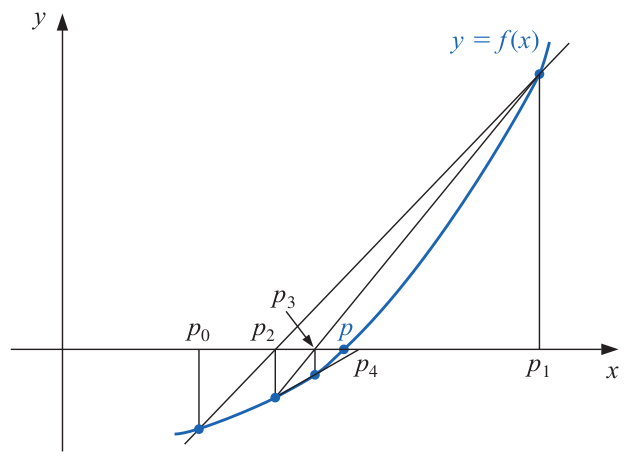
\includegraphics[width=.5\textwidth]{fig/secantes.png}
    \legend{Fonte: \cite{numerical-anal-burden}}
    \label{f-metodo-secante}
\end{figure}

Sintetizando o comportamento descrito com base no proposto por \citeauthor{numerical-anal-burden} no \autoref{alg-sec-orig}:


\begin{algorithm}[H]
\caption{Método clássico das secantes}\label{alg-sec-orig}
\begin{algorithmic}[1]

\Require Pontos iniciais e finais $a,b$ ; Tolerância TOL; Número máximo de iterações $N_0$
\Ensure Solução $c$ para $f(c) = 0$ ou erro

\State $F_A \gets f(a)$ \Comment{$F_A$ recebe o valor da função no ponto}
\State $F_B \gets f(b)$
\State $i \gets 2$ \Comment{\textit{flag} de iteração é inicializada}
\While{$i \leq N_0$}

    \State $c \gets b - F_B \cdot \frac{b-a}{F_B - F_A}$ \Comment{Calcula o ponto de intersecção com a abcissa}
    \State $F_C \gets f(c)$

    \If{$|c - b| < $ {TOL}}
        \State \textbf{return}(c)
    \EndIf

    \State $i \gets i + 1$
    
    \State $a\gets b$
    \State $b \gets c$
    \State $F_A \gets F_B$
    \State $F_B \gets f(c)$ \Comment{Novo cálculo para a próxima reta secante}
\EndWhile
\State \textbf{return} "Method failed"
\end{algorithmic}
\legend{Fonte: Adaptado de \cite{numerical-anal-burden}}
\end{algorithm}

O método das secantes torna-se uma solução razoável no cenário de implementação em software e hardware onde não é possível calcular uma derivada analítica da função avaliada, como propõe o método de Newton. Uma vez que a secante oferece uma aproximação adequada da derivada no ponto por iteração, o ponto calculado caminha em direção à raiz.

\subsection{Método das secantes com seleção de intervalo}

O terceiro método estudado é na verdade uma adaptação do método das secantes. Este terceiro método, chamado de "Secante modificada"\; ou "Secante com seleção de intervalos"\; é apenas uma forma mais eficiente de selecionar o intervalo de busca baseando-se nas propriedades da curva de $Q \times I_{REF}$. A motivação para a formalização deste terceiro método veio enquanto testava-se o algoritmo desenvolvido do método das secantes e observou-se alta sensibilidade às condições iniciais. Algo que aconteceu de forma menos expressiva comparando-se com o método da bisseção.

O método da secante com seleção de intervalo foi considerado uma formalização à parte ao invés de somente uma adaptação, pois como elencado por \citeauthor{numerical-anal-burden}, há métodos que seguem exatamente a mesma ideia de outros já formalizados e são considerados outro método por melhorarem a razão de convergência.

Alguns exemplos de métodos que aplicam alguma modificação em um método clássico são os métodos de Aitken $\Delta^2$ e Steffensen, que visam construir uma sequência $c_n$ que convirja mais rapidamente modificando o cálculo das secantes. Outros exemplos tomam como base propriedades da função a ser aproximada (se é um polinômio, se há zeros complexos, etc) e reduzem a quantidade de iterações com base na especialização do método. 

Dessa forma, introduz-se uma seleção de intervalos no método das secantes à partir da observação do comportamento da curva de  $Q \times I_{REF}$ dando destaque às suas duas regiões na \autoref{f-q-iref-regioes}.

\begin{figure}[H]
    \centering
    \caption{$Q \times I_{REF}$ com destaque para as regiões linear e não linear}
    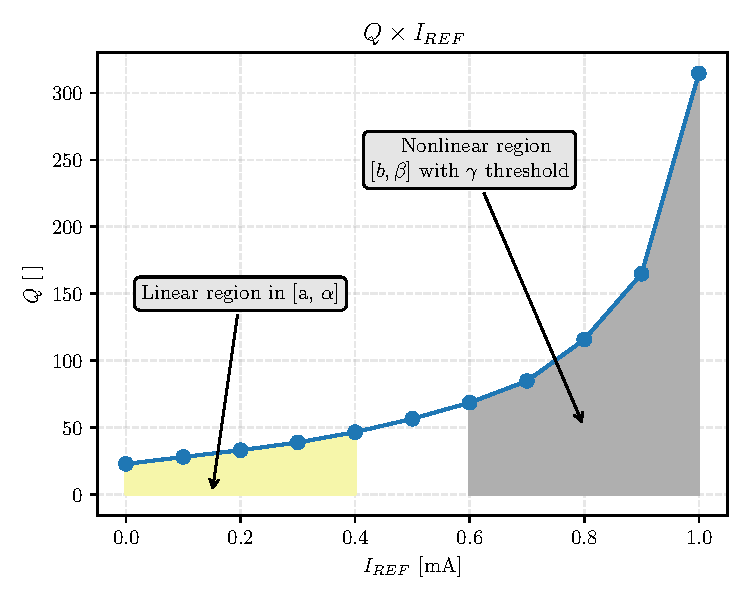
\includegraphics[width = .7\textwidth]{fig/q-iref-regions.pdf}
    \label{f-q-iref-regioes}
\end{figure}

Da \autoref{f-q-iref-regioes} dá-se destaque para duas regiões: Uma onde o $Q$ varia de forma aproximadamente linear com o aumento de $I_{REF}$ (região sombreada de amarelo entre 0 e 0.4mA) e outra onde o $Q$ varia de forma mais abrupta se comparada com a região linear. Com este comportamento pode-se particionar a busca em dois intervalos distintos, um entre [a, $\alpha$] e outro entre [$\beta$, b].

Existe uma faixa intermediária [$\alpha, \beta$] que aparenta inicialmente não integrar a busca. De fato na primeira iteração não integra, mas, da segunda em diante, quando é calculado o ponto $c$, esta faixa passa a integrar o intervalo de busca. Essa faixa intermediária é ajustável de acordo com os parâmetros $[\alpha, \beta]$. O parâmetro $\gamma$ ajusta o \textit{threshold} da busca. A partir de $Q_d > \gamma $ é usada a região de busca $[b, \beta]$. Caso contrário usa-se $[a, \alpha]$.



\chapter{Metodologia}

\section{Adaptação de métodos numéricos para busca de valores}\label{sec-adapt-metodos}

Como citado anteriormente e descrito no \autoref{ch-referencial} -- \nameref{ch-referencial}, os métodos numéricos para aproximação de funções não-lineares são projetados originalmente para encontrar raízes. Entretanto, a adaptação para a busca de valores pode ser feita mantendo as características originais dos métodos modificando a maneira como alguns cálculos são feitos e suas condições de parada. 

A primeira modificação feita é a inserção da variável a ser buscada ($Q_d$). Este é o valor de $Q$ que o usuário almeja obter. Outra modificação é que agora o algoritmo não controla internamente o número de iterações\footnote{Nos testes do \autoref{ch-res} é usada uma variável auxiliar MAX\_ITER apenas para restringir o testbench.} $i$.


A inicialização dos valores para o intervalo de busca também é feita de forma diferente pela condição de instabilidade da curva $Q \times I_{REF}$ como mencionado no \autoref{ch-referencial}. O limite inferior de corrente sempre será 0mA enquanto o superior é passado como parâmetro para o algoritmo, sendo este $I_{Stable}$.


Outra modificação relevante é que o algoritmo agora se assemelha mais à um procedimento do que de uma função, pois não retorna valores, apenas retém os valores de corrente. Essa modificação foi implementada para alinhar o comportamento do algoritmo tanto em  hardware quanto em software.

As subseções \autoref{ss-adapt-bis} a \autoref{ss-adapt-modsec} descrevem as adaptações feitas para a busca de valores. É introduzida também a corrente de referência -- $I_{REF}$ para ilustrar chamadas ao bloco de medição.

\subsection{Método da bisecção}\label{ss-adapt-bis}

No método da bisseção, as modificações mais importantes são a condição de parada e a seleção do próximo valor. No algoritmo original, é usado  o  teorema do valor intermediário para seleção do próximo intervalo [a,b] de busca \cite{numerical-anal-burden}. Como na busca de valores pode não haver a troca de sinal, substitui-se o retorno em caso de $f(c) \approx 0 \vee f(c) < $ TOL pela diferença entre o $Q$ medido e o desejado. Caso essa diferença seja menor que a tolerância, considera-se que o algoritmo convergiu.

Em caso de ainda não ter alcançado a convergência, a seleção dos novos valores é feita de forma similar mas sem usar o teorema do valor intermediário: caso o erro ($\varepsilon$) seja negativo, indica que o valor procurado está entre o intervalo [c, b]. Caso contrário está entre [a, c]. A transcrição do algoritmo adaptado desenvolvido é visível no \autoref{alg-bi}.

\begin{algorithm}[H]
\caption{Método adaptado da bisseção}
\begin{algorithmic}[1]

\Require TOL, $Q_{d}$, $Q_{m}$, $I_{Stable}$
\Ensure $I_{REF} \; | \; \varepsilon \leq$ TOL

\State $a \gets 0$
\State $b \gets I_{Stable}$
\State Converged $\gets$ \textbf{False}
 
\While{not Converged}

    \State $c \gets \frac{a+b}{2}$
% \Comment{$I_{REF}$ is updated to "c"\; value}

    \State $I_{REF} \gets c$ 

    \State $Q_{m} \gets Q_{m}\left(I_{REF}\right)$ \Comment{Realiza-se uma medição do $Q$ com o novo valor de $I_{REF}$}

    \State $\varepsilon \gets Q_m - Q_d $

    \If{$\varepsilon \leq $ TOL} Converged $\gets$ \textbf{True} 
        \Else
            \If{$\varepsilon > 0$}
                \State $a \gets c$
            \EndIf
            \If{$\varepsilon < 0$}
                \State $b \gets c$
            \EndIf
    \EndIf

\EndWhile
\end{algorithmic}
\label{alg-bi}
\end{algorithm}

A atribuição feita na linha 7 do \autoref{alg-bi} é feita apenas para simbolizar que há uma atualização do valor de $Q_m$ assim que um novo $I_{REF}$ é atribuído na linha anterior. Foi escolhido representar essa atribuição, pois em software ela é somente uma chamada de função que acontece instantaneamente, mas em hardware é uma operação de medição que requer alguns ciclos de \textit{clock}, portanto, não é uma atribuição instantânea.

O método mantém as mesmas características de convergência do original, uma vez que foram modificadas apenas operações atômicas, mantendo sua ordem de convergência linear.

\subsection{Método das secantes}\label{ss-adapt-sec}

Para o método das secantes, a estratégia de encontrar o próximo ponto $c$ que intersecciona o eixo $x$ é simples: translada-se a curva com o valor $Q_d$. Em outras palavras, $c$ é calculado da mesma forma e diminui-se o valor de $Q_d$ para que a raiz da curva seja $f(c) = Q_d$ ao invés de zero. 


A atribuição de $c$ é repartida em duas instruções diferentes. Primeiro calcula-se a inclinação da reta secante (Linha 6 do \autoref{alg-sec}) e depois calcula-se o ponto de intersecção com a reta transladado pelo valor de $Q$ desejado (Linha 8 do \autoref{alg-sec}). 

As instruções foram separadas pois percebe-se que os valores da inclinação podem pequenos, resultando em divisão por zero e potenciais estouros de memória em hardware. Verificando o valor da variável antes de calcular e atribuir à $c$, pode-se evitar valores indefinidos.

Para a condição de convergência basta calcular se o erro ($\varepsilon$) entre o valor medido e o desejado está aceitável conforme a tolerância escolhida. Neste caso é calculado o valor absoluto pois a posterior atribuição dos novos intervalos não necessita do sinal de $\varepsilon$ como no \nameref{alg-bi}. O método adaptado desenvolvido é visível no \autoref{alg-sec}.

\begin{algorithm}[H]
\caption{Método adaptado das secantes}\label{alg-sec}
\begin{algorithmic}[1]

\Require TOL, $Q_{d}$, $Q_{m}$, $I_{Stable}$
\Ensure $I_{REF} \; | \; \varepsilon \leq$ TOL

\State $a \gets 0$
\State $b \gets I_{Stable}$
\State Converged $\gets$ \textbf{False}

\While{not Converged} \\

    \State slope $ \gets \dfrac{Q_m(b) - Q_m(a)}{b-a}$ \Comment{$Q_m(a), Q_m(b)$ são novas medições} \\
    \State $c \gets b - \dfrac{Q_m(b) - Q_d}{\text{slope}}$
    \State $I_{REF} \gets c$

    \State $Q_{m} \gets Q_{m}\left(I_{REF}\right)$  \Comment{Medição do $Q$ com o novo valor de $I_{REF}$}

    \State $\varepsilon \gets \left|Q_m - Q_d \right|$

    \If{$\varepsilon \leq $ TOL} Converged $\gets$ \textbf{True} 
        \Else
            \State $a \gets b$
            \State $b \gets c$
    \EndIf

\EndWhile
\end{algorithmic}
\end{algorithm}

Diferentemente da busca por raiz, na busca por valores não é necessário que os valores de medição fossem reatribuídos em caso de não-convergência, como faz o \autoref{alg-sec-orig} nas linhas 12-13.

Como comentado no próprio código, $Q_m(a)$ é uma nova chamada de medição com $I_{REF} = a$. Nota-se que no método das secantes há três chamadas desse tipo para o bloco de medição em cada iteração ($Q_m(a), Q_m(b), Q_m(c)$). Como a operação de medição é a operação que mais leva ciclos de \textit{clock} para completar, considera-se um ponto de atenção ao comparar-se o desempenho dos algoritmos desenvolvidos em HDL.


\subsection{Método das secantes com seleção de intervalo}\label{ss-adapt-modsec}

O método das secantes com seleção de intervalo segue as mesmas considerações feitas adaptando o \autoref{alg-sec-orig} para o \autoref{alg-sec}. Durante a execução, a determinação dos valores de coeficientes ($\alpha, \beta, \gamma$) que selecionam a região de intervalo é feita com base na curva de $Q \times I_{REF}$ conforme mostrado no \autoref{ch-referencial}, \autoref{f-q-iref-regioes}. O método adaptado desenvolvido é visível no \autoref{alg-sec-mod}:

\begin{algorithm}[H]
\caption{Método adaptado das secantes com seleção de intervalo desenvolvido}\label{alg-sec-mod}
\begin{algorithmic}[1]

\Require TOL, $Q_{d}$, $Q_{m}$, $I_{Stable}$
\Ensure $I_{REF} \; | \; \varepsilon \leq$ TOL

\State Converged $\gets$ \textbf{False}
\State $Q_{max} \gets Q_m(I_{Stable})$
\If{$Q_d > \gamma \cdot Q_{max}$} \Comment{Seleção na região linear}
    \State $a \gets \alpha \cdot I_{Stable}$
    \State $b \gets I_{Stable}$
    \Else \Comment{Seleção na região não-linear}
        \State $a \gets 0$
        \State $b \gets \beta \cdot I_{Stable}$
\EndIf


\While{not Converged}  \\
    \State slope $ \gets \dfrac{Q_m(b) - Q_m(a)}{b-a}$
    \Comment{$Q_m(a), Q_m(b)$ são novas medições} \\
    \State $c \gets b - \dfrac{Q_m(b) - Q_d}{\text{slope}}$
    \State $I_{REF} \gets c$

    \State $Q_{m} \gets Q_{m}\left(I_{REF}\right)$  \Comment{Medição do $Q$ com o novo valor de $I_{REF}$}

    \State $\varepsilon \gets \left|Q_m - Q_d \right|$

    \If{$\varepsilon \leq $ TOL} Converged $\gets$ \textbf{True} 
        \Else
            \State $a \gets b$
            \State $b \gets c$
    \EndIf

\EndWhile
\end{algorithmic}
\end{algorithm}

Além das considerações sobre as chamadas feitas ao bloco de medição e as mesmas considerações relativas ao método original, o método modificado é baseado em experimentação. Dessa forma, sempre haverá margem para otimização na escolha dos coeficientes. Um problema de otimização à parte.



\section{Arquitetura do sistema}\label{sec-arquitetura}

 Em linhas gerais, a arquitetura deve responder à um único requisito funcional: O usuário entra com um valor decimal para o $Q$ desejado e o sistema deve retornar o valor de corrente referente à este valor de $Q$ desejado. \autoref{f-arq-sys} ilustra a arquitetura desenvolvida com todas\footnote{Todos os blocos têm um \textit{reset} assíncrono, não representado para simplificação} as entradas, saídas e blocos correspondentes ao circuito proposto:

\begin{figure}[H]
    \centering
    \caption{Arquitetura desenvolvida para o sistema}
    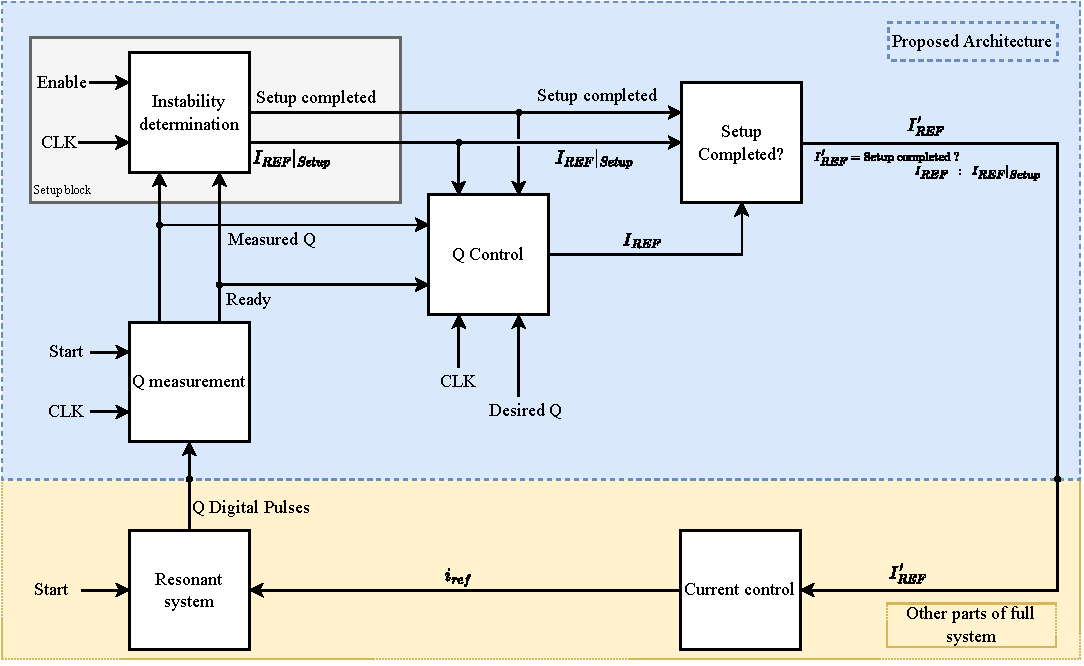
\includegraphics{fig/tcc-nova-arq.pdf}
    \label{f-arq-sys}
\end{figure}

O cenário base de funcionamento em um ciclo completo desde a inicialização até ter atingido o valor de $Q$ desejado é elencado da seguinte forma:

\begin{enumerate}
    \item O sistema inicializa variáveis internas e prossegue para a determinação do valor máximo de corrente de referência de configuração ($I_{REF_|{Setup}}$) conforme justificado posteriormente na \autoref{ss-instability-determination} -- \nameref{ss-instability-determination}.
    \item O bloco de determinação de instabilidade manipula a corrente de configuração do sistema até determinar onde é o ponto máximo de estabilidade. O valor da corrente é atualizado sempre que recebe uma nova medição do bloco de medição do $Q$ à cada ciclo de \textit{clock} até atingir o ponto de estabilidade.
    \item Com o limite superior de corrente determinado, este valor é passado ao bloco de controle como valor máximo de corrente a ser injetada no sistema ressonante. Neste momento o bloco $Q\; control$ está livre para manipular a corrente $I_{REF}$ para alcançar o fator-Q desejado, logo, habilita-se o bloco de controle do Q. O valor de corrente injetada é atualizado sempre que recebe uma nova medição do bloco de medição do $Q$.
    \item Após o alcançar o Q desejado, o sistema mantém o valor de corrente para o bloco que a controla, mantendo este estado até receber uma nova solicitação de um valor de $Q$ desejado.
\end{enumerate}

As partes subsequentes (\autoref{ss-medição-q} -- \autoref{ss-q-control}) descrevem o funcionamento bloco a bloco individualmente e no que diz respeito à comunicação entre blocos.

Vale ressaltar que, apesar de serem desenvolvidos três métodos de controle do fator de qualidade, apenas um é testado por vez (e posteriormente o projeto avançará apenas com o método de melhor desempenho com relação à todo o sistema).

\subsection{Medição do $Q$: $Q$ \textit{measurement}}\label{ss-medição-q}

A medição do $Q$ é um passo fundamental que acaba por coordenar os demais blocos. Essa responsabilidade de coordenação dá-se pela característica de que os pulsos emitidos pelo sistema ressonante (\textit{Q digital pulses}) não ``avisam'' que a medição do $Q$ terminou, como ilustra a \autoref{f-timing-q-measurement}. Sendo assim, este bloco é responsável por temporizar a operação dos blocos subsequentes pois faz interface direta com o sistema ressonante. O diagrama de temporização da \autoref{f-timing-q-measurement} ilustra o comportamento do bloco que mede o valor de $Q$:

\begin{figure}[H]
    \centering
    \caption{Diagrama de tempo da operação do bloco de medição.}
    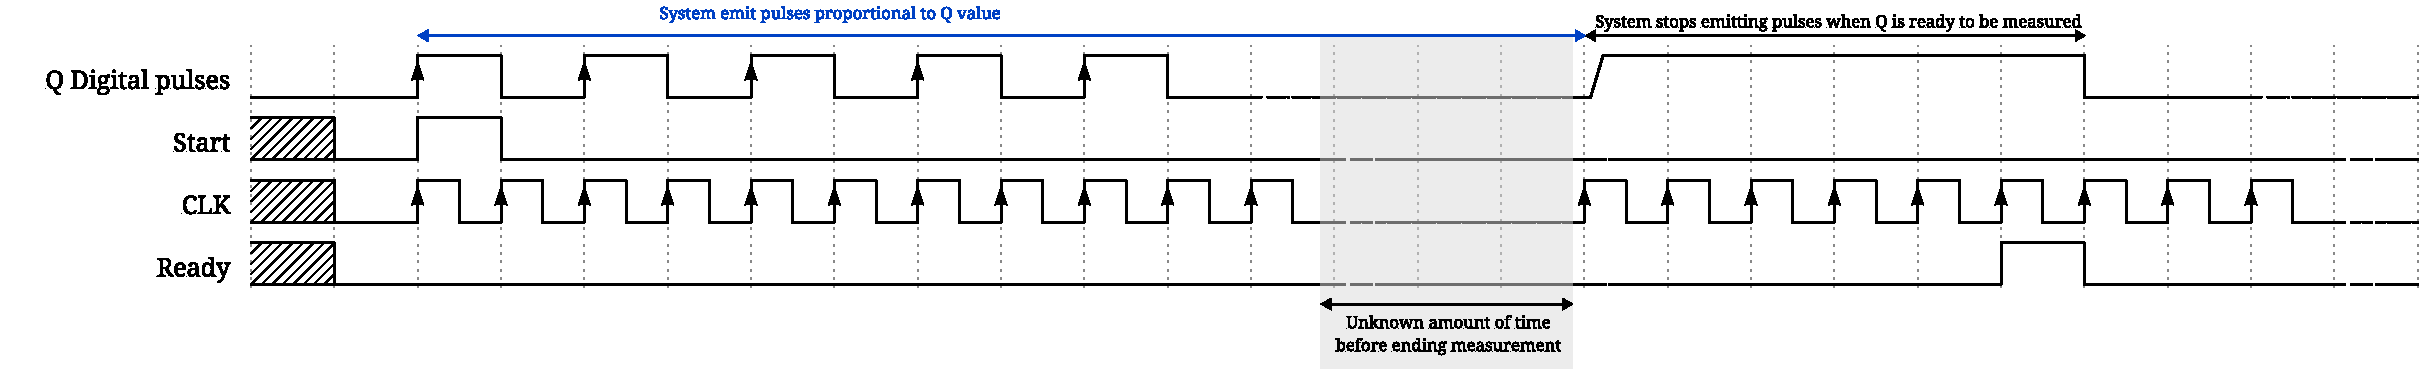
\includegraphics{fig/timing-q-measurement.pdf}
    \legend{Fonte: o autor}
    \label{f-timing-q-measurement}
\end{figure}

O sistema ressonante emite $n$ pulsos continuamente por um período de tempo indeterminado\footnote{O período mínimo e máximo são conhecidos uma vez que os valores mínimos e máximos de $Q$ são medidos} proporcional ao $Q$ até detectar que a medição está completa. Neste momento, para-se de emitir pulsos e  congela-se o valor lógico alto indicando que a medição terminou. Como não há nenhuma \textit{\textit{flag}} emitida pelo sistema ressonante para indicar que a medição está pronta, implementa-se uma estratégia de contador que aciona a \textit{flag} \textit{ready} gerada pelo bloco de medição.

Para detectar que a medição está completa e levar à nível alto a \textit{flag} "\textit{ready}"\; incrementa-se um contador interno à cada Ciclo de \textit{clock}. Caso no ciclo seguinte o valor do pulso esteja alto, incrementa-se esse contador. Caso seja baixo, reseta-se. A \textit{flag} \textit{ready} é setada como "1"\; quando o valor do contador atinge o valor decimal 5. Assim, este contador age como um temporizador que ``espera'' os pulsos acabarem por 5-CC para indicar que a medição terminou e setar a \textit{flag} \textit{ready}. Este valor foi obtido empiricamente, abrindo margem para futura otimização.


\subsection{Determinação de limite de instabilidade: \textit{Instability determination}}\label{ss-instability-determination}

O comportamento da curva $Q \times I_{REF}$, conta com uma característica na qual a partir de certo ponto de corrente o $Q$ tende ao infinito e cai abruptamente a partir dese ponto com o aumento da corrente. Desta forma é necessário determinar o ponto máximo de estabilidade do sistema à fim de não ultrapassar a região de estabilidade no momento de fazer a busca do fator de qualidade desejado. Este ponto está destacado na \autoref{f-timedomain-q-iref-qmax-istable}:

\begin{figure}[H]
    \centering
    \caption{Curva $Q \times I_{REF}$ com destaque para o ponto máximo de estabilidade}
    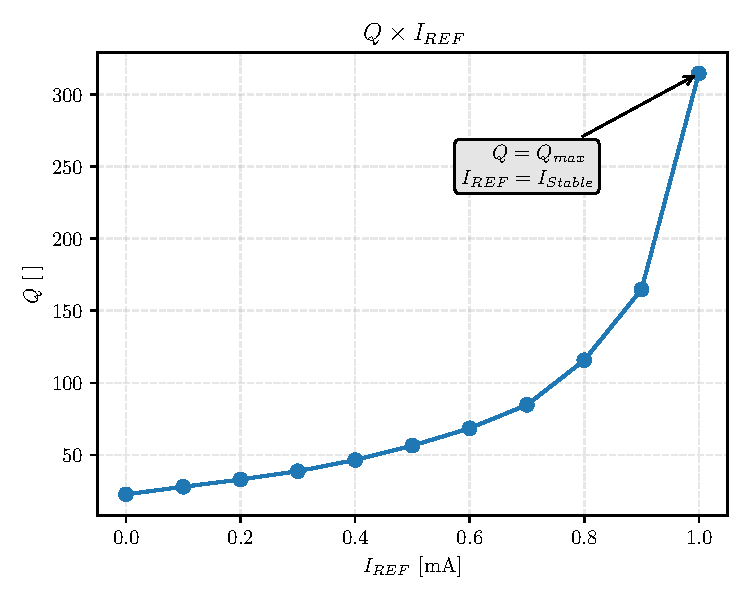
\includegraphics[width=.7\textwidth]{fig/q-iref-q_max-i_stable.pdf}
    \legend{Fonte: o autor}
    \label{f-timedomain-q-iref-qmax-istable}
\end{figure}


Para encontrar limite de instabilidade, sendo o ponto $p = (I_{Stable}, Q_{Máx})$ o bloco em questão opera conforme o algoritmo: \autoref{alg-instability}:

\begin{algorithm}[H]
\caption{Algoritmo de determinação de instabilidade}\label{alg-instability}
\begin{algorithmic}[1]

\Require{$\Delta Q, \Delta I_{REF}$, $Q_m$}
\Ensure{$I_{Stable}$} 

\State $I_{Stable} \gets I_{MAX}$ \Comment{$I_{MAX} =$ 1mA}
\State Found $\gets$ \textbf{False}

\While{not Found}
    
    \State $Q_i \gets Q_m(I_{Stable})$
    \State $I_{Stable} \gets I_{Stable}  - \Delta I_{REF}$
    \State $Q_{i+1} \gets Q_m(I_{Stable})$
    \If{$\left(Q_{i+1} - Q_i \geq \Delta Q\right)$}
        \State Found $\gets$ \textbf{True}
    \EndIf
\EndWhile
\State \textbf{return $I_{Stable}$}
\end{algorithmic}
\legend{Fonte: o autor}
\end{algorithm}



% Expĺicar a porra do algoritmo

No domínio do tempo, vale lembrar que a medição do fator de qualidade não é instantânea e depende da \textit{\textit{flag}} \textit{ready} do bloco de medição. O diagrama de temporização da \autoref{f-timing-instability-determination} ilustra o comportamento: 

% faz requisições contínuas para o bloco de medição até detectar um $\uparrow\Delta Q$ abrupto para determinado $\Delta I_{REF}$ partindo do pressuposto que na região instável o $Q$ medido é mais baixo que o $Q$ máximo do atingível. O diagrama de temporização da \autoref{f-timing-instability-determination} ilustra o comportamento:

% O \autoref{alg-instability-determination} exemplifica a estratégia adotada de detecção de \delta$Q$

% Como mostrado no \autoref{alg-instability-determination}, o mesmo decrementa o valor de corrente de referência até detectar um $\Delta Q$ suficientemente alto para detectar

\begin{figure}[H]
    \centering
    \caption{Diagrama de tempo da operação do bloco de determinação de instabilidade}
    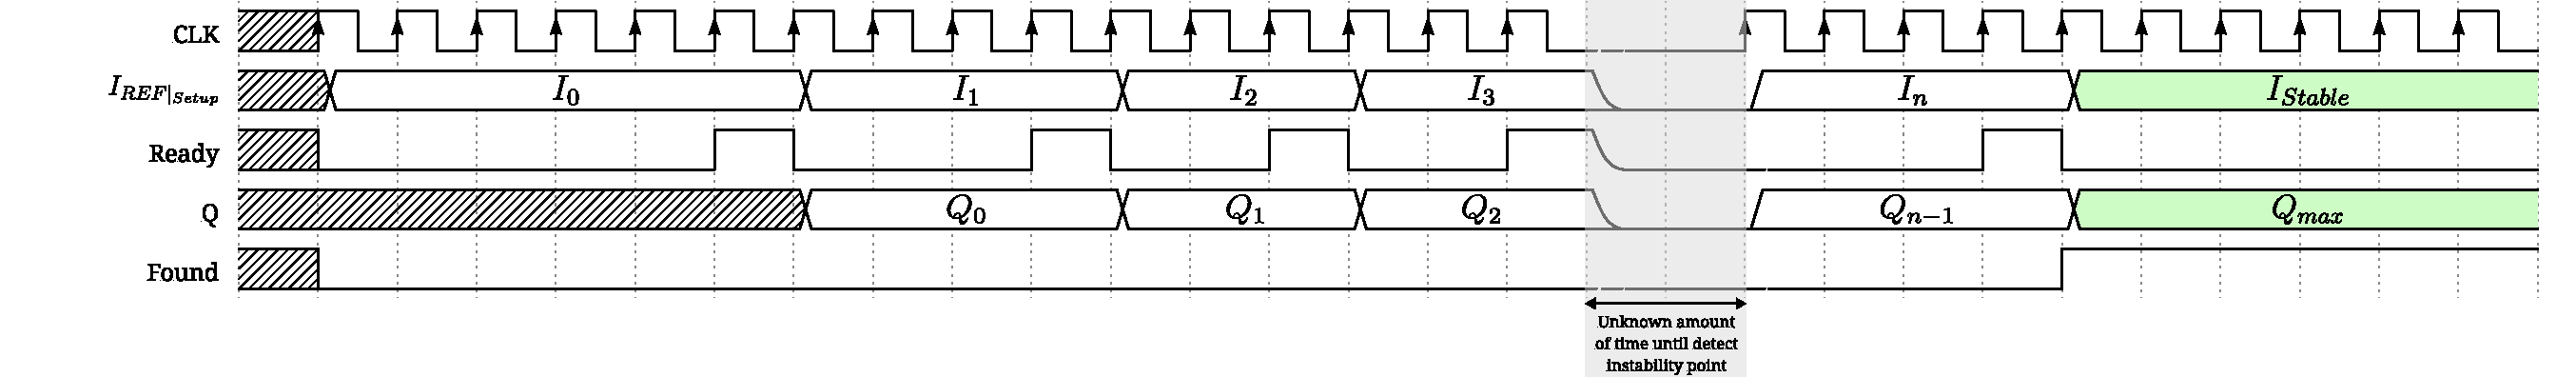
\includegraphics{fig/timing-instability-determination.pdf}
    \legend{Fonte: o autor}
    \label{f-timing-instability-determination}
\end{figure}

Alinhando \autoref{alg-instability} com a \autoref{f-timing-instability-determination}, tem-se que na corrente inicial $I_0$ (corrente máxima do sistema) é decrementado o valor $\Delta I_{REF}$ passado como parâmetro do algoritmo até que o decremento de corrente produza um $\Delta Q$ maior ou igual ao parâmetro especificado, atingindo assim o ponto $p = (I_{Stable}, Q_{Máx})$. Quando este ponto é alcançado um registrador interno \verb|Found| é setado para 1, indicando que o ponto está determinado e a operação de configuração finalizada. Neste momento o bloco de controle do $Q$ está livre para atuar.

% O \autoref{alg-instability} 




% Talvez citar a otimização do ponto máximo de $Q$ definido

% A \autoref{f-timedomain-q-iref-qmax-istable} dá destaque o para as as variáveis $I_{Stable}$ e $Q_{Máx}$ (ponto de limite de estabilidade) ilustradas no diagrama de temporização da \autoref{f-timing-instability-determination}:


\subsection{Seleção de correntes: \textit{Setup completed}}\label{ss-seleção-correntes}

Este bloco é essencialmente um multiplexador $2\times 1$ com $N = 10$ bits em cada canal de entrada (e saída) na via principal de dados usados no sistema. A \autoref{f-bloco-setup-completed} ilustra a simplificação deste bloco:

\begin{figure}[H]
    \centering
    \caption{Representação do bloco intertravamento ou seleção de correntes}
    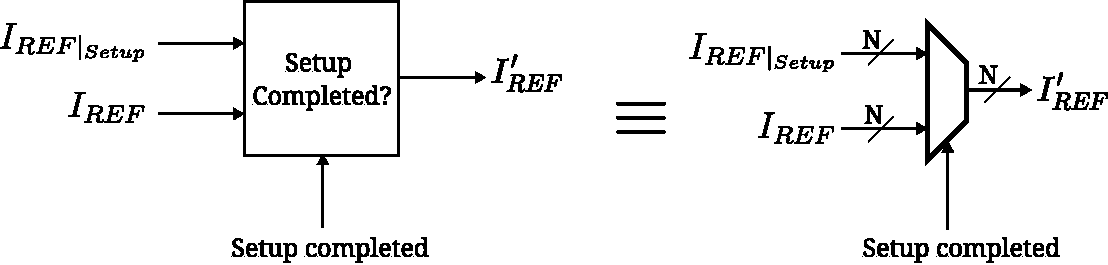
\includegraphics[width=.9\textwidth]{fig/setup-completed-equiv.pdf}
    \label{f-bloco-setup-completed}
\end{figure}

Esse bloco garante que apenas uma das correntes seja injetada ao mesmo tempo no sistema ressonante. Esta seleção entre $I_{REF}|_{setup}$ e $I_{REF}$ se faz necessária devido a necessidade de determinar primeiramente a corrente máxima do circuito ressonante ($I_{REF}|_{setup}$). Após esta determinação, o circuito digital poderá efetuar a busca pelo $Q$ desejado sendo $I_{REF}|_{setup}$ o limite superior de corrente, pois após este ponto, o sistema se encontrará em instabilidade.


O bloco \textit{Setup Completed?} possui uma variável seleção de 1 bit chamada \textit{Setup completed} e faz a multiplexação dos sinais $I_{REF}|_{setup}$ e $I_{REF}$ para a saída $I_{REF}'$. Enquanto esta variável de seleção estiver em nível lógico baixo, o bloco \textit{Instability Determination} buscará o valor máximo de $Q$ e, portanto, faz com que a saída $I_{REF}'$ receba a informação de $I_{REF}|_{setup}$. A variável de seleção somente ficará em nível lógico alto quando o valor máximo de $Q$ for determinado, assim, permitindo que a saída $I_{REF}|_{setup}$ receba a informação de $I_{REF}$ para a convergência do $Q$ desejado através do bloco \textit{$Q$ Control}. A sua saída ($I_{REF}'$) É resultado da variável de seleção (\textit{Setup completed}).

As formas de onda ilustradas na \autoref{f-timing-iref-selection} exemplificam um ciclo de funcionamento da fase de configuração para a fase de controle e manipulação da corrente:%

\begin{figure}[H]
    \centering
    \caption{Diagrama de tempo da operação do bloco de seleção de corrente}
    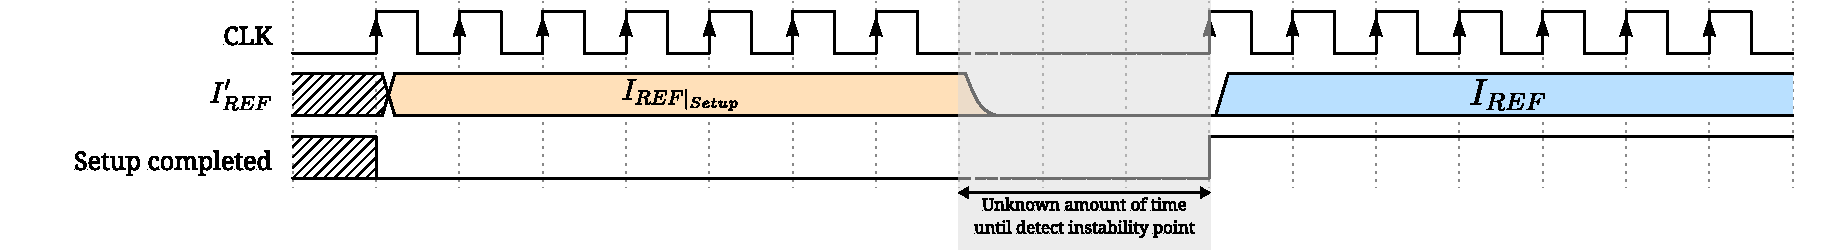
\includegraphics{fig/timing-iref-selection.pdf}
    \legend{Fonte: o autor}
    \label{f-timing-iref-selection}
\end{figure}

Da \autoref{f-timing-iref-selection} infere-se que há um primeiro momento onde a corrente de configuração é injetada até que seja determinado um valor máximo de corrente para manter a estabilidade. Quando isto ocorre a \textit{\textit{flag}} \textit{Setup completed} recebe o valor "1"\; e então o sistema está apto a controlar a corrente para receber o $Q$ desejado.



\subsection{Controle do Q: $Q$ \textit{Control}}\label{ss-q-control}

Quando o sistema já tem determinado qual o limite superior de corrente a fim de não atingir a instabilidade (\autoref{ss-instability-determination}), o bloco \textit{$Q$ control} é ativado para controlar a corrente Iref e buscar o Q desejado inserido pelo usuário.

Retomando o que foi mencionado nos \nameref{ch-obj}, neste projeto foram implementados 3 métodos principais mencionados na \autoref{sec-adapt-metodos}. O bloco de controle em si contém e executa apenas um método por vez, não sendo possível alternar entre métodos uma vez compilado o código e executadas as simulações. O sistema é projetado desta forma pois o objetivo é selecionar o método com melhor desempenho acerca de todo o sistema e prosseguir para o fluxo de fabricação.

O diagrama de temporização deste bloco (\autoref{f-timing-q-control}) é bastante similar ao do bloco de determinação de instabilidade (\autoref{f-timing-instability-determination}).

\begin{figure}[H]
    \centering
    \caption{Diagrama de tempo da operação do bloco de controle do $Q$.}
    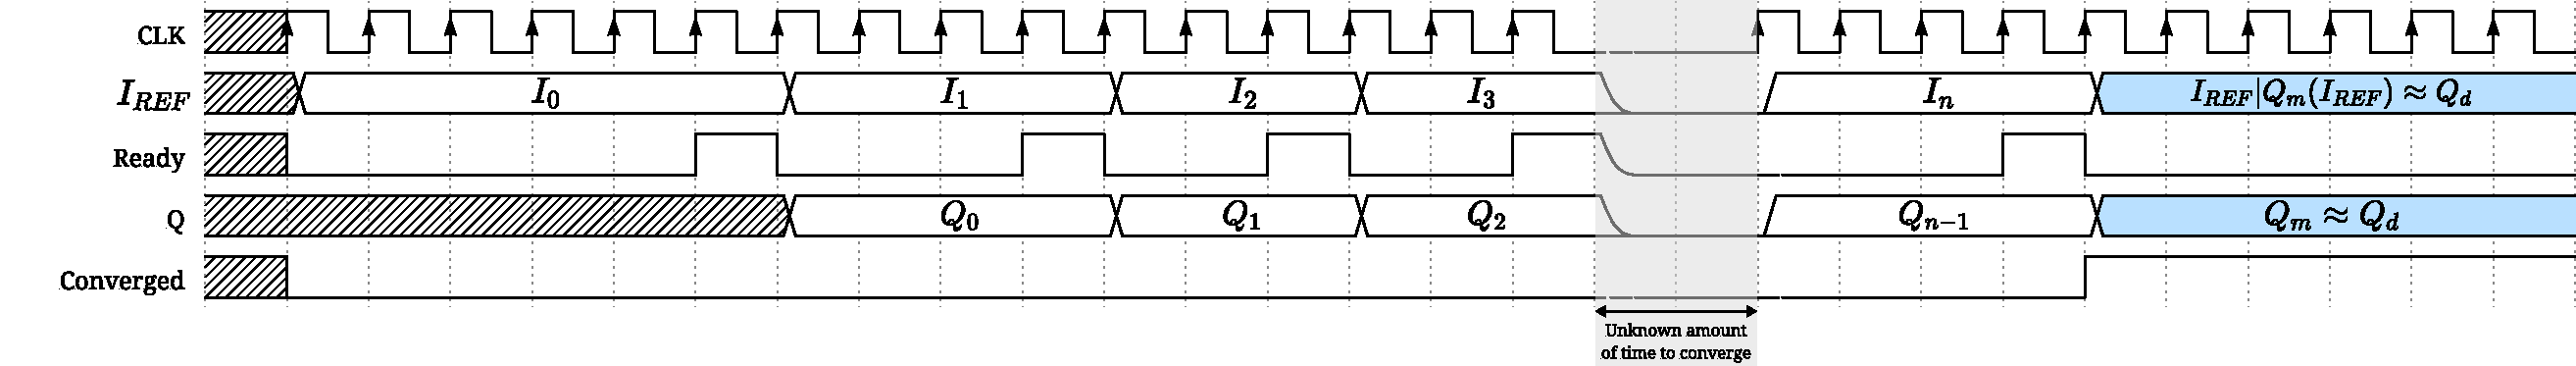
\includegraphics{fig/timing-q-control.pdf}
    \legend{Fonte: o autor}
    \label{f-timing-q-control}
\end{figure}

Para cada método de controle o diagrama de temporização pode variar brevemente no que diz respeito ao número de ciclos de \textit{\textit{clock}} para terminar uma operação e no \textit{overhead} inicial. Por exemplo, o método das secantes necessita de 3 medições de $Q$ para a primeira comparação enquanto o da bisseção necessita somente de duas. 




% \subsubsection{Considerações sobre implementação em \textit{hardware}}




\section{Arquitetura de testes do sistema}

A arquitetura de testes foi desenvolvida para validar individualmente cada módulo do sistema. Como há comunicação entre os módulos desenvolvidos e o sistema ressonante, o \textit{testbench} foi abstraído em 3 elementos, representados na \autoref{f-arq-tb-simplif}:

\begin{figure}[H]
    \centering
    \caption{Arquitetura dos \textit{testbenches}}
    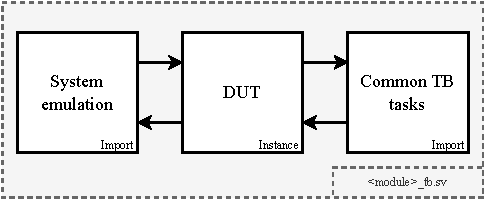
\includegraphics[width=.5\textwidth]{fig/simplif-tb-structure.pdf}
    \label{f-arq-tb-simplif}
\end{figure}

Da \autoref{f-arq-tb-simplif} há 3 elementos presentes em cada arquivo de \textit{testbenching} que diz respeito à cada módulo \verb|<module>_tb.sv|, sendo eles:

\begin{enumerate}
    \item DUT -- Módulo: O módulo a ser testado com respectivas conexões
    \item \textit{System emulation} -- Package: É um pacote a ser importado no \verb|<module>_tb.sv| com as funcionalidades referentes à emulação do comportamento do sistema ressonante. Em sua maioria é apenas a geração dos $Q$ \textit{digital pulses} à partir de um start, como ilustrado na \autoref{f-arq-simplif} -- \nameref{f-arq-simplif}
    \item \textit{Common TB tasks} -- Package: É outro com funcionalidades comuns à tesbenches: geração de \textit{clock}, monitoramento de variáveis, entrada e saída de dados para arquivos. 
\end{enumerate}

A arquitetura de testes foi projetada desta forma para testar os módulos desenvolvidos na \nameref{f-arq-sys} de forma independente e promover o reuso de funções em comum. Com essa estrutura é possível testar todos os módulos desenvolvidos, adequando apenas os cenários de teste, adequando apenas o arquivo principal \verb|<module>_tb.sv|.

Nesta fase do projeto todos os módulos foram testados seguindo a estrutura mencionada ao longo desta seção. Em um segundo momento, como mencionado no \autoref{ch-obj} -- \nameref{ch-obj} os blocos serão testados de forma conjunta, verificando a sincronia e os e a coerência dos resultados obtidos do sistema acoplado \textit{versus} blocos independentes.


% Para tal, há 3 \textit{pools} ou seções de módulos em cada arquitetura, com as seguintes responsabilidades:

% \begin{enumerate}
%     \item \textit{Main modules}: Instanciar cada módulo da arquitetura e permitir a comunicação com as variáveis de seu respectivo testbench.
%     \item \textit{Independent TB modules}: Instanciar o módulo a ser testado e importar as funções de teste e de emulação do sistema. Este pool contem um testbench para cada módulo real do sistema e é responsável por conter a instância real de cada módulo
%     \item [\textit{Reusable features}]:
% \end{enumerate}

% Para a arquitetura de testes do sistema, em um primeiro momento, testam-se os módulos de forma independente a fim de verificar seu funcionamento. Como estes módulos apesar de terem um funcionamento distinto entre si, são projetados para trabalhar em conjunto (Vide \autoref{f-arq-sys}). Esta arquitetura de testes (Fig. \ref{f-arq-tb}) permite verificar o funcionamento do sistema independente da sincronia, que por si só, exige um testbench à parte.

% \begin{figure}[H]
%     \centering
%     \caption{Arquitetura desenvolvida para os \textit{testbenches}}
%     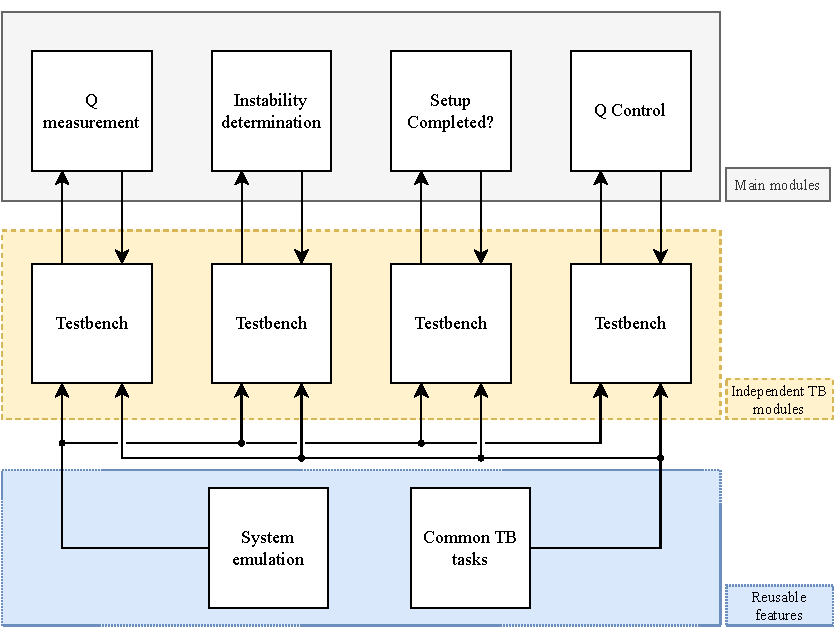
\includegraphics[width=.9\textwidth]{fig/tcc-tesbench-structure.pdf}
%     \label{f-arq-tb}
% \end{figure}

% Na \autoref{f-arq-tb} os módulos contidos no \textit{pool} de testes ``\textit{main modules}'' são nada mais que instâncias dos módulos da arquitetura construída (\autoref{f-arq-sys}). Como estes módulos estão acoplados e comunicam entre si, o módulo auxiliar ``\textit{System emulation}'' emula o comportamento do sistema de acordo com um cenário específico de testes, replicando o comportamento dos módulos que interagem. Em outras palavras, o bloco \textit{System emulation} foi pensado como um aparato de DFT auxiliar na verificação do comportamento do sistema em partes independentes. 

% A comunicação do DUT com as outras partes do sistema é responsabilidade de cada bloco de testbench no pool ``\textit{Independent TB modules}''. Além disso, o instanciamento de cada módulo e importação das funcionalidades pertinentes ao teste do \textit{System emulation} é feito dentro do testbench individual para cada módulo

% O bloco ``Common TB tasks'' abstrai funcionalidades em comum à todos os testbenches, como por exemplo: geração de \textit{clock}s, leitura e escrita de arquivos e captura de dados, funções de debug e ec.





% Além de separar as responsabilidades de testes, a arquitetura permite o reuso de funções em comum de testbenches, como exemplos:

% \begin{itemize}
%     \item Geração de \textit{clock}
%     \item Leitura de arquivos e parseamento de dados
%     \item Captura de dados
%     \item Inserçaõ de cenários diferentes de testes
% \end{itemize}


\chapter{Resultados e análise}\label{ch-res}

Nesta fase do projeto, foram implementados e validados individualmente dois dos blocos principais: bloco de controle do $Q$ e bloco de determinação de instabilidade.

No bloco de determinação de instabilidade a implementação foi feita diretamente em HDL. Para os métodos de aproximação foram primeiro prototipados em alto nível e na sequência transcritos para HDL, comparando-se o resultado entre métodos e entre implementações

\section{Resultados do bloco de determinação do limite de estabilidade}

Para o teste de determinação do ponto máximo de estabilidade foi modificada a curva padrão de $Q \times I_{REF}$ utilizada em todo trabalho de forma sintética, isto é, foram alterados os dados para que o ponto de instabilidade estivesse localizado no ponto (índice) 850 de $I_{REF} = 0.83$mA. A curva modificada consta na \autoref{f-inst-test}:

\begin{figure}[H]
    \centering
    \caption{Dados teóricos e sintéticos utilizados para o teste de determinação de instabilidade}
    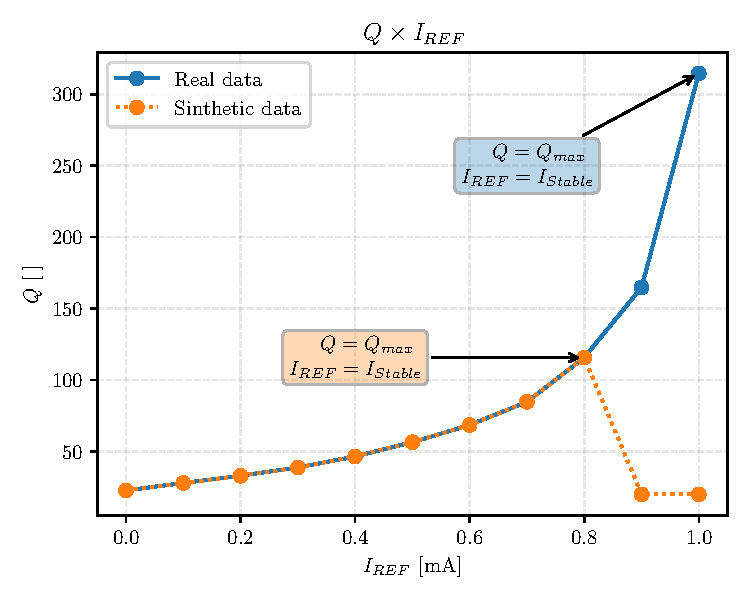
\includegraphics[width=.5\textwidth]{fig/q-iref-instability-test.pdf}
    \label{f-inst-test}
    \legend{Fonte: o autor}
\end{figure}

Os dados sintéticos foram usados em virtude de que, se fossem usados os dados reais, o algoritmo encontraria o ponto logo na primeira operação, uma vez que o ponto onde $I_{REF} = 1$mA é o ponto máximo de estabilidade. 


Testa-se o bloco com os parâmetros da \autoref{tab-spec-inst} e os resultados são visíveis na \autoref{tab-teste-inst}:

\begin{table}[H]
    \centering
    \caption{Parâmetros passados ao algoritmo de determinação de instabilidade}
    \resizebox{\textwidth}{!}{%
\begin{tabular}{lll}
\hline
\textbf{Parâmetro}& \textbf{Valor} & \textbf{Descrição}                            \\ \hline
$\Delta Q$                              & 50 [ ]                             & Variação de $Q$ considerada suficiente para sair da região instável \\
$\Delta I_{REF}$                        & 10 [bits]                          & Valor de decremento da corrente de configuração                     \\
$p = (I_{Stable}, Q_{max})$            & (850 [bits], 113 [ ])              & Ponto (definido) de estabilidade                                    \\
MAX\_ITER                               & 50                                 & Numero máximo de iterações. (neste caso são ciclos de clock)        \\ \hline
\end{tabular}%
}
    \label{tab-spec-inst}
     \legend{Fonte: o autor}
\end{table}

\begin{table}[H]
    \centering
    \caption{Resultados da busca por ponto máximo de estabilidade.}
    \begin{tabular}{rrrr}
\toprule
 Time &  $I_{REF}$ [bits] &  $Q_m$ &  $I_{REF}$ [mA] \\
\midrule
    2 &   1013 &   23 &    0.989258 \\
    7 &    993 &   23 &    0.969727 \\
   12 &    963 &   23 &    0.940430 \\
   17 &    943 &   23 &    0.920898 \\
   22 &    913 &   23 &    0.891602 \\
   27 &    893 &   23 &    0.872070 \\
   32 &    863 &   23 &    0.842773 \\
   36 &    843 &   113 &   0.823242 \\
\bottomrule
\end{tabular}

    \label{tab-teste-inst}
     \legend{Fonte: o autor}
\end{table}

Da \autoref{tab-teste-inst} verifica-se que o ponto de estabilidade é determinado como 843 enquanto o esperado é 850 após 
36 ciclos de \textit{clock}. Como os parâmetros de $\Delta I_{REF}, \Delta Q$ foram ajustados priorizando a proximidade com o ponto definido (850). Pode-se priorizar a rapidez da busca em troca de obter um $Q_{max}$ menor ajustando os parâmetros.


\section{Resultados do bloco de controle do $Q$}

O bloco de controle do $Q$ foi testado em dois cenários: o padrão, onde a tolerância é coerente com os valores de $Q$ produzidos; o sintético, onde a tolerância é baixa. Foram testados os 3 métodos em alto nível e o método da bisseção em HDL.

% Os resultados dos dois métodos das secantes foram testados em valores;


\subsection{Algoritmos em alto nível}%
Primeiro, realiza-se um teste busca de um valor único seguindo as especificações da \autoref{tab-spec-single}. Os valores elencados na \autoref{tab-spec-single} foram selecionados de forma que o teste representasse um cenário real de uma busca única. Os valores mínimos e máximos de corrente foram definidos de acordo com as capacidades do sistema ressonante, o valor de tolerância de acordo com a resolução do sistema de medição e o número máximo de iterações fixado em 32 para o caso de algum método não alcançar convergência.%
\begin{table}[H]
    \centering
    \caption{Especificações do teste de busca por valor único}
    \begin{tabular}{@{}lll@{}}
\toprule
\textbf{Parâmetro} & \textbf{Valor} & \textbf{Descrição}                   \\ \midrule
$a$                & 0.0            & Limite inferior inicial de $I_{REF}$ \\
$b$                & 1.0            & Limite superior inicial de $I_{REF}$ \\
TOL                & $\pm 30$       & Tolerância ou erro máximo admissível \\
$Q_d$              & 110            & Valor de Q desejado                  \\
MAX\_ITER           & 32             & Numero máximo de iterações.          \\ \bottomrule
\end{tabular}
    \label{tab-spec-single}
    \legend{Fonte: o autor}
\end{table}

Executando o teste com os parâmetros da \autoref{tab-spec-single} para cada método desenvolvido em alto nível, têm-se os resultados para cada método na \autoref{tab-res-single} em suas respectivas sub-tabelas.

\begin{table}[H]%
    \centering
    \caption{Resultados de execução do teste de busca única para cada método, $Q_d = 110$.}
    \begin{subtable}[H]{\textwidth}
        \centering
        \caption{Bisseção}
        \begin{tabular}{cccccc}
\toprule
Iteração & $a$ & $b$ &  $c$ &    $f(c)$ & $\varepsilon$ \\
\midrule
       1 & 0.0 & 1.0 & 0.50 & 56.743276 &    -53.256724 \\
       2 & 0.5 & 1.0 & 0.75 & 98.171202 &    -11.828798 \\
\bottomrule
\end{tabular}

        % \vspace{10pt}
    \end{subtable}
    \begin{subtable}[H]{\textwidth}
        \centering
        \caption{Secante}
        \begin{tabular}{cccccc}
\toprule
Iteração &      $a$ &      $b$ &      $c$ &      $f(c)$ & $\varepsilon$ \\
\midrule
       1 & 0.000000 & 1.000000 & 0.299006 &   38.839856 &    -71.160144 \\
       2 & 1.000000 & 0.299006 & 0.479866 &   54.497986 &    -55.502014 \\
       3 & 0.299006 & 0.479866 & 1.120945 & 1623.460030 &   1513.460030 \\
       4 & 0.479866 & 1.120945 & 0.502544 &   57.028494 &    -52.971506 \\
       5 & 1.120945 & 0.502544 & 0.523456 &   59.379481 &    -50.620519 \\
       6 & 0.502544 & 0.523456 & 0.973731 &  248.961601 &    138.961601 \\
       7 & 0.523456 & 0.973731 & 0.643685 &   74.313694 &    -35.686306 \\
       8 & 0.973731 & 0.643685 & 0.711124 &   87.462432 &    -22.537568 \\
       9 & 0.643685 & 0.711124 & 0.826718 &  126.652723 &     16.652723 \\
      10 & 0.711124 & 0.826718 & 0.777600 &  107.326038 &     -2.673962 \\
      11 & 0.826718 & 0.777600 & 0.784396 &  109.773166 &     -0.226834 \\
\bottomrule
\end{tabular}

        % \vspace{10pt}
    \end{subtable}
    \begin{subtable}[H]{\textwidth}
        \centering
        \caption{Secante modificada}
        \begin{tabular}{cccccc}
\toprule
Iteração & $a$ & $b$ &    $c$ &     $f(c)$ & $\varepsilon$ \\
\midrule
       1 & 0.8 & 1.0 & 0.7943 & 113.472012 &      3.472012 \\
\bottomrule
\end{tabular}

        % \vspace{10pt}
    \end{subtable}
    \legend{Fonte: o autor}
    \label{tab-res-single}
\end{table}%
Dos dados obtidos com uma busca de valor percebe-se que a secante modificada e a secante clássica comportam-se de forma diferente apesar de serem baseados no mesmo algoritmo, simplesmente por escolher o intervalo de busca de maneira diferente. Assim, o algoritmo original apresentou o pior desempenho dos três, sendo o da bisseção o com desempenho intermediário. Sintetizando essa busca em um gráfico , na \autoref{f-res-single} vê-se a aproximação do $Q$ para o valor desejado:%

% \vspace*{-1.6cm}
\begin{figure}[H]
    \centering
    \caption{Pontos obtidos por iteração e curva $Q \times I_{REF}$ dos métodos de busca em alto nível}
    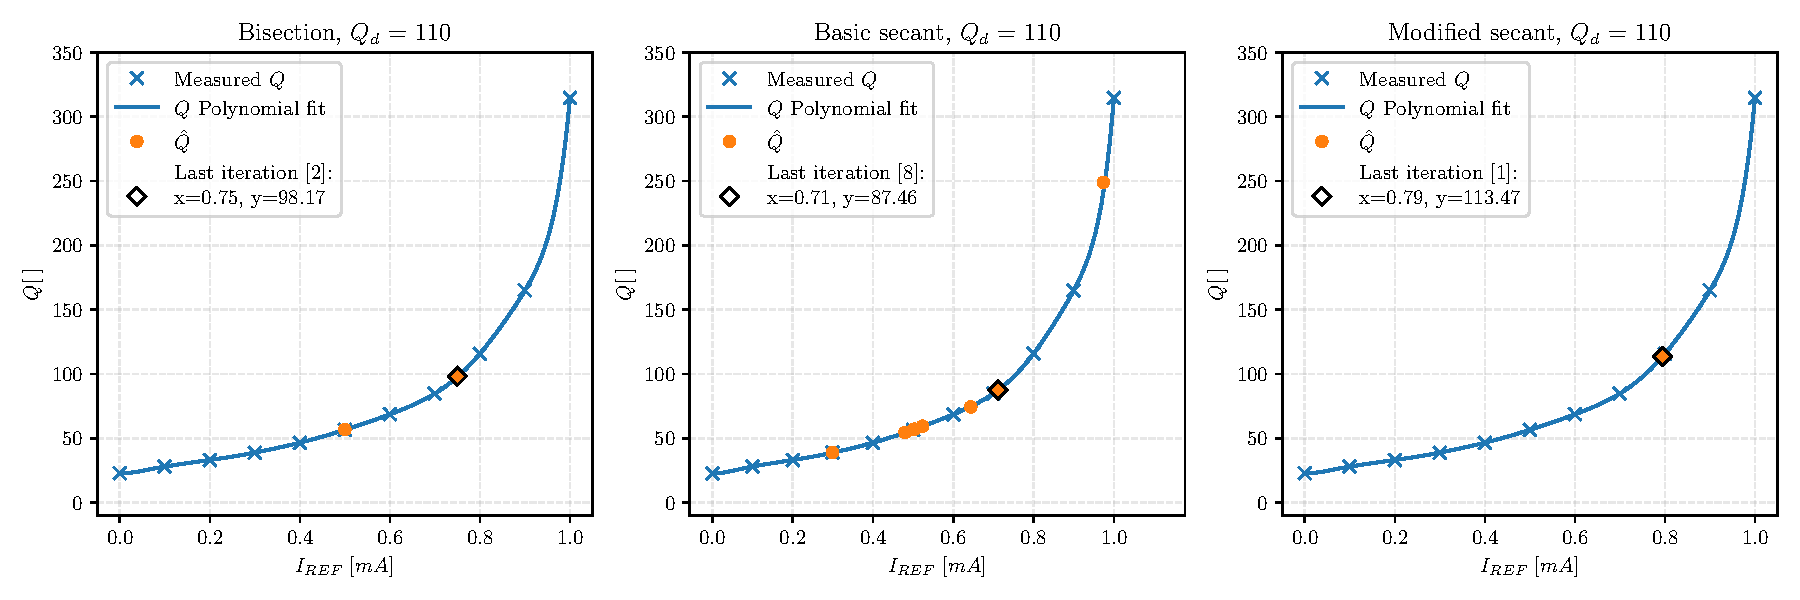
\includegraphics{fig/res-methods-single.pdf}
    \legend{Fonte: o autor}
    \label{f-res-single}
\end{figure}


Para um teste mais abrangente foi feito um  \textit{sweeep} de valores de $Q$ desejado ($Q_d$) e medido quantas iterações foram necessárias para que o algoritmo viesse a convergir. As especificações do teste são visíveis na \autoref{tab-spec-sweep}: 

\begin{table}[H]
    \centering
    \caption{Especificações do teste de busca em \textit{sweep}}
    \begin{tabular}{@{}lll@{}}
\toprule
\textbf{Parâmetro} & \textbf{Valor} & \textbf{Descrição}                   \\ \midrule
$a$                & 0.0 [mA]            & Limite inferior inicial de $I_{REF}$ \\
$b$                & 1.0 [mA]            & Limite superior inicial de $I_{REF}$ \\
TOL                & $\pm 30$       & Tolerância ou erro máximo admissível \\
$Q_d$              & 30 até 300 com passo de 20           & Valor de Q desejado                  \\
MAX\_ITER           & 32             & Numero máximo de iterações.          \\ \bottomrule
\end{tabular}
     \legend{Fonte: o autor}
    \label{tab-spec-sweep}
\end{table}

Os resultados do teste com as especificações da \autoref{tab-spec-sweep} são visíveis na \autoref{fig-itc-q-trend} em conjunto com um ajuste polinomial de $Q_d \times$ ITC:

\begin{figure}[H]
    \centering
    \caption{Número de iterações para convergência e valor desejado de $Q$ com alta tolerância}
    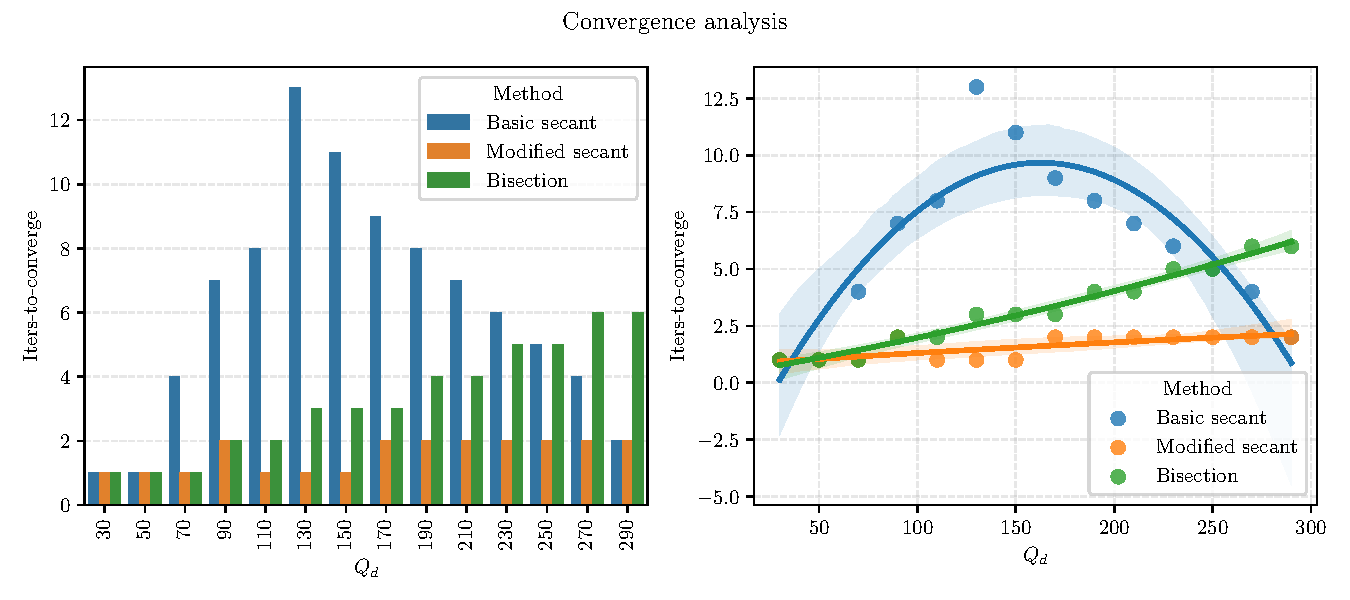
\includegraphics{fig/conv-analysis-no-drop.pdf}
     \legend{Fonte: o autor}
    \label{fig-itc-q-trend}
\end{figure}

Na \autoref{fig-itc-q-trend} verifica-se um desempenho razoável para todos os métodos, porém, o método da secante com seleção de intervalo apresentou melhor desempenho, enquanto o da secante básica, o pior.

Um comportamento que se destaca pelas linhas de tendência do gráfico é que tanto a secante modificada quanto o método da bisseção têm sua ordem de convergência aproximadamente linear enquanto a secante básica apresenta uma característica parabólica negativa. Em outras palavras, a secante básica demora mais para convergir quando o $Q_d$ está localizado no ponto central da curva de $Q \times I_{REF}$. A bisseção e a secante modificada demoram mais enquanto o ponto está mais próximo do valor máximo atingível. A \autoref{tab-stats-sweep} apresenta algumas estatísticas sobre cada método.

\begin{table}[H]
    \centering
    \caption{Tabela com mínimo, máximo, média, desvio e variância de ITC por método}
        \begin{tabular}{lrrrrr}
\toprule
{} &              Min &              Max &              Mean &               STD &               VAR \\
{} & ITC & ITC & ITC & ITC & ITC \\
\midrule
Basic secant    &                 1 &                13 &          6.142857 &          3.591810 &         12.901099 \\
Bisection       &                 1 &                 6 &          3.285714 &          1.772811 &          3.142857 \\
Modified secant &                 1 &                 2 &          1.571429 &          0.513553 &          0.263736 \\
\bottomrule
\end{tabular}

    \legend{Fonte: o autor}
    \label{tab-stats-sweep}
\end{table}

Na média, a secante básica requer o dobro de iterações para convergência se comparado com o da bisseção, que por sua vez também requer aproximadamente o dobro da secante modificada. Os valores máximos seguem o mesmo padrão. Os valores mínimos acabam por ser iguais devido a alta tolerância. O desvio segue a tendência da média indicando baixa dispersão.


\subsubsection{Cenário sintético com baixa tolerância}

O teste em \textit{sweep} foi repetido com menor tolerância, para investigar se os métodos são capazes de alcançar a convergência em um cenário sintético onde o $Q_m$ pudesse ser medido com maior resolução. As especificações são essencialmente as mesmas da \autoref{tab-spec-sweep} com exceção da tolerância que agora é $\pm 1$
Os resultados do teste sintético são visíveis na \autoref{fig-itc-q-trend-low-tol} em conjunto com um ajuste polinomial de $Q_d \times$ ITC:

\begin{figure}[H]
    \centering
    \caption{Número de iterações para convergência e valor desejado de $Q$ com baixa tolerância}
    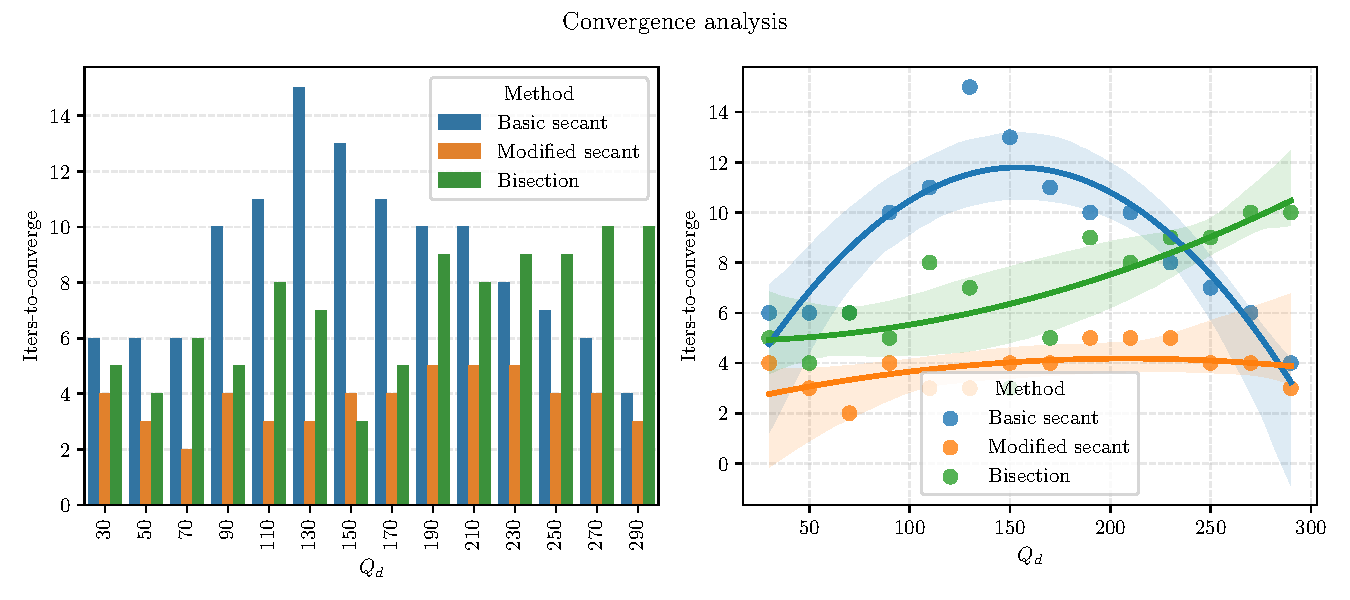
\includegraphics{fig/conv-analysis-no-drop-low-tol.pdf}
     \legend{Fonte: o autor}
    \label{fig-itc-q-trend-low-tol}
\end{figure}

Na \autoref{fig-itc-q-trend-low-tol} verifica-se o mesmo padrão encontrado no cenário realista de testes (Resultados da \autoref{fig-itc-q-trend}), onde a tolerância é mais alta. O método da secante com seleção de intervalo manteve-se com o melhor desempenho,  entretanto, com uma característica que agora mais se assemelha à uma parábola com concavidade negativa. O método da bisseção continua a sendo o método intermediário mas agora com um formato parabólico positivo. O método da secante básica manteve exatamente as mesmas características. Na \autoref{tab-stats-sweep-low-tol} estão resumidas algumas estatísticas dos métodos:

\begin{table}[H]
    \centering
    \caption{Tabela com mínimo, máximo, média, desvio e variância de ITC por método}
        \begin{tabular}{lrrrrr}
\toprule
{} &              Min &              Max &              Mean &               std &               var \\
{} & ITC & ITC & ITC & ITC & ITC \\
\midrule
Basic secant    &                 4 &                15 &          8.785714 &          3.142233 &          9.873626 \\
Bisection       &                 3 &                10 &          7.000000 &          2.320477 &          5.384615 \\
Modified secant &                 2 &                 5 &          3.785714 &          0.892582 &          0.796703 \\
\bottomrule
\end{tabular}

 \legend{Fonte: o autor}
    \label{tab-stats-sweep-low-tol}
\end{table}

Agora, na média, a secante básica não requer mais o dobro de iterações para convergência se comparado com o da bisseção: a secante básica é $1.25\times$ mais lenta. No caso da bisseção com a secante modificada, a diferença ainda é alta, sendo aproximadamente $1.85\times$ mais lenta. Os valores mínimos são relativamente próximos enquanto os máximos apresentam diferença de 1.5$\times$ e de $2\times$ comparando o melhor método com o intermediário, e o intermediário com o pior, respectivamente. O desvio padrão e a variância são mais altos nos casos da secante básica e da bisseção se comparados com a secante modificada, indicando alta dispersão.


\subsection{Algoritmos em HDL}

Para os algoritmos em HDL testa-se somente o cenário sintético, uma vez que sendo capazes de alcançar convergência com baixa tolerância, também serão capazes de alcançar com menor exigência de precisão.

Os dois métodos das secantes não foram testados num cenário abrangente, pois, apesar de terem sido desenvolvidos, apresentaram problemas de convergência quando implementados em HDL. Estes problemas ocorreram no cálculo da inclinação da reta secante e posterior atribuição do valor de $c$. 

Se retomarmos o cálculo da inclinação da reta dos algoritmos \ref{alg-sec} e \ref{alg-sec-mod}, percebe-se que este pode envolver valores próximos de 0. No momento que $0 \leq $ \textit{slope} $ < 1$ essa variável recebe o valor de 0 pois a resolução usada é de 1 bit. Esse arredondamento é um problema neste contexto pois gera divisão por zero, então o método atribui um valor indefinido ('$x$' em hardware) para $c$, que faz com que o método fique estagnado em um valor de corrente.

Para tentar contornar o problema, no algoritmo desenvolvido foi usada uma atribuição condicional para caso a inclinação recebesse o valor de 0. Apesar de convergir para alguns valores, o método torna-se instável e não converge para outros valores. Desta forma, mostra-se nos resultados um exemplo onde foi possível atingir a convergência e outro onde não foi.

\subsection{Resultados do método da bisseção}

Repete-se o teste sintético com os parâmetros da \autoref{tab-spec-single} para a busca de valor único exceto pela tolerância de $\pm 1$ para um $Q_d = 110$. O resultado dessa é visto na \autoref{tab-res-single-bisect}.

\begin{table}[H]
    \centering
    \caption{Pontos obtidos por iteração no método da bisseção}
        \begin{tabular}{ccc}
\toprule
$I_{REF}$ [bits] & $I_{REF} \; [mA]$ & $Q_m$ \\
\midrule
                511 &          0.499511 &    56 \\
                767 &          0.749756 &    97 \\
                895 &          0.874878 &   151 \\
                831 &          0.812317 &   121 \\
                799 &          0.781036 &   108 \\
                815 &          0.796676 &   114 \\
                807 &          0.788856 &   111 \\
                803 &          0.784946 &   110 \\
\bottomrule
\end{tabular}

         \legend{Fonte: o autor}
    \label{tab-res-single-bisect}
\end{table}

Construindo um gráfico com os pontos da \autoref{tab-res-single-bisect} verifica-se na \autoref{f-res-single-bisect} que o método converge para mais perto do valor desejado à cada iteração até atingir o ponto onde $TOL \leq Q_m - Q_d$.

\begin{figure}[H]
    \centering
    \caption{Gráfico dos pontos obtidos por iteração no método da bisseção}
    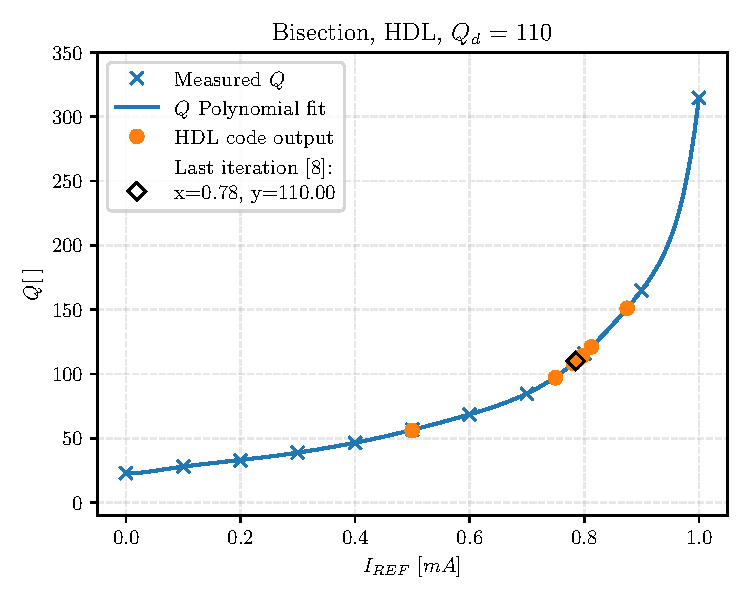
\includegraphics[width=.5\textwidth]{fig/res-bisect-single-hdl.pdf}
     \legend{Fonte: o autor}
    \label{f-res-single-bisect}
\end{figure}





% \textcolor{red}{pq q tem isso aqui, eu esqueci}
% \begin{figure}[H]
%     \centering
%     \caption{Pontos obtidos por iteração e curva $Q \times I_{REF}$ do método da bisseção em HDL}
%     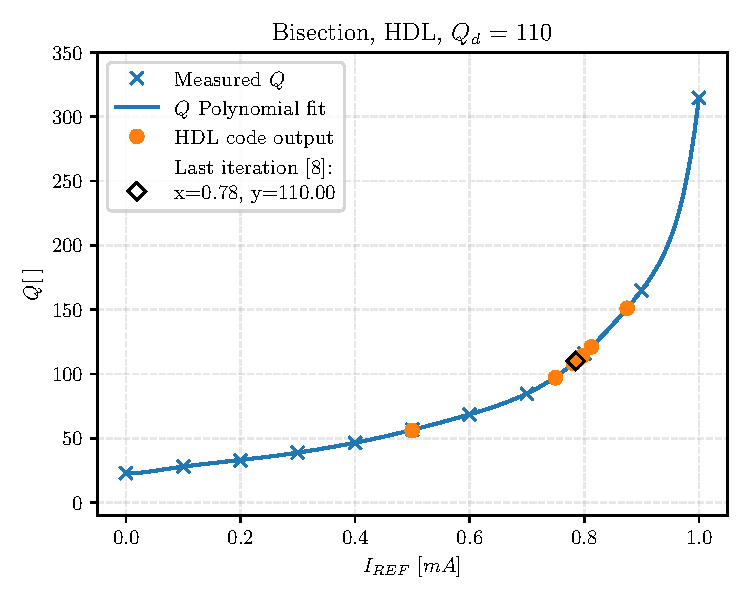
\includegraphics[width=.5\textwidth]{fig/res-bisect-single-hdl.pdf}
%     \label{fig:enter-label}
% \end{figure}

Realiza-se também um \textit{sweep} de valores assim como feito para os algoritmos em alto nível. Neste teste compara-se o desempenho do método da bisseção implementado em linguagem de programação (PL) \textit{versus} sua versão em linguagem de descrição de hardware (HDL). Esses resultados são visíveis na \autoref{f-itc-q-trend-low-tol-bisect}.


\begin{figure}[H]
    \centering
    \caption{Número de iterações para convergência \textit{versus} $Q_d$ do método da bisseção em de HDL \textit{versus} PL}
    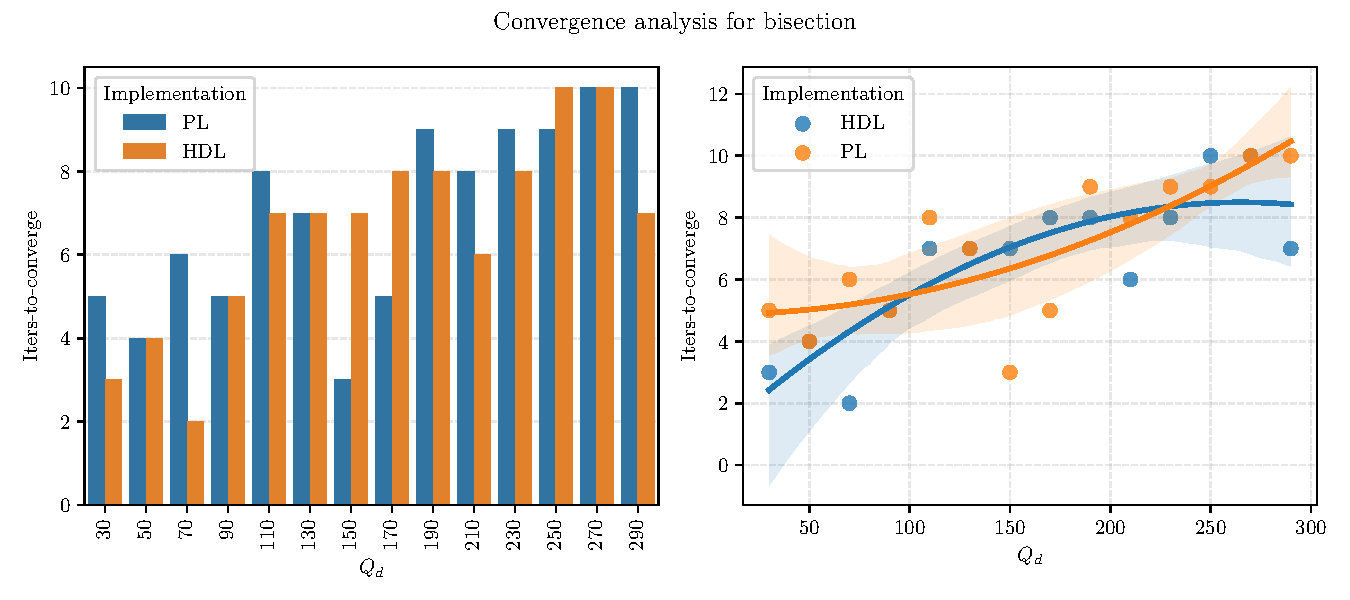
\includegraphics{fig/conv-analysis-no-drop-bisect.pdf}
     \legend{Fonte: o autor}
    \label{f-itc-q-trend-low-tol-bisect}
\end{figure}

Verifica-se na \autoref{f-itc-q-trend-low-tol-bisect}, que os algoritmos implementados em hardware e software têm seu desempenho similar. As diferenças surgem pelos arredondamentos e aritmética de ponto flutuante: em software são usados 6 dígitos após a virgula para valores de $c (I_{REF})$ resultando em $\pm 1nA$ de precisão -- de fato exagerado. Enquanto em hardware, em conversão direta são usados valores inteiros num range de 0 a 1023, resultando em $\approx 0.97\mu$A de precisão. Essa variação de precisão por vezes fez com que o método implementado em PL fosse mais lento com que sua versão em HDL. Em linhas gerais, o desempenho é o mesmo. Resumindo as estatísticas da busca em \textit{sweep} na \autoref{tab-stats-low-tol-bisect}.

\begin{table}[H]
    \centering
    \caption{Tabela com mínimo, máximo, média, desvio e variância de ITC por implementação}
        \begin{tabular}{lrrrrr}
\toprule
{} &              amin &              amax &              mean &               std &               var \\
{} & Iters-to-converge & Iters-to-converge & Iters-to-converge & Iters-to-converge & Iters-to-converge \\
Implementation &                   &                   &                   &                   &                   \\
\midrule
HDL            &                 2 &                10 &          6.571429 &          2.376626 &          5.648352 \\
PL             &                 3 &                10 &          7.000000 &          2.320477 &          5.384615 \\
\bottomrule
\end{tabular}

     \legend{Fonte: o autor}
    \label{tab-stats-low-tol-bisect}
\end{table}

Na \autoref{tab-stats-low-tol-bisect} percebe-se estatísticas similares por implementação. Enquanto os valores máximos são iguais, os valores mínimos e médios são menores para a versão em HDL dados pela menor precisão. Por sua vez, desvio e variância são ligeiramente menores em PL.

Por último, representa-se a busca em sweep feita para o método da bisseção em HDL na \autoref{f-sweep-bisect}. Neste gráfico, espera-se que os valores produzidos pelo algoritmo (Circulos vermelhos -- $\hat{Q}$) em sweeep reconstruam a forma da curva.

\begin{figure}[H]
    \centering
    \caption{Busca em sweep dos valores de $Q$ no método da bisseção}
    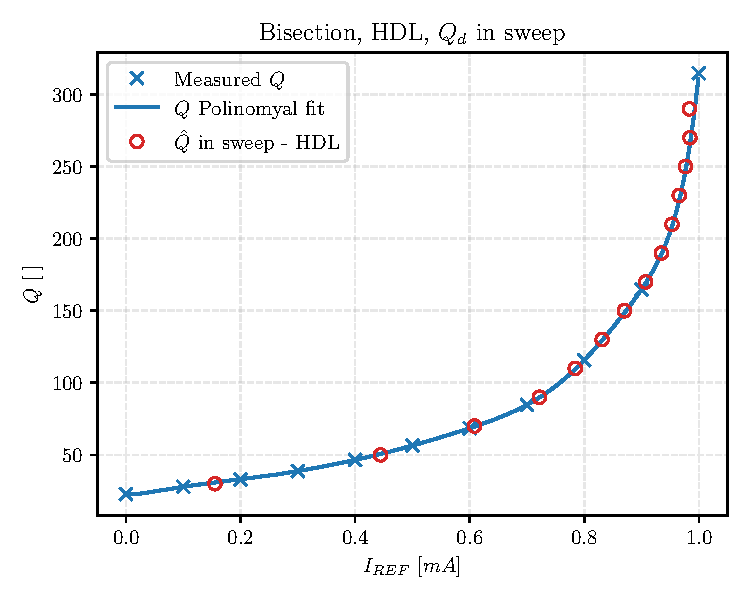
\includegraphics[width=.5\textwidth]{fig/res-bisect-sweep-hdl.pdf}
     \legend{Fonte: o autor}
    \label{f-sweep-bisect}
\end{figure}

Percebe-se que os pontos aproximados estão suficientemente próximos do $Q_d$ com a alta precisão requerida ao algoritmo.

\subsection{Resultados do método das secantes}

Como comentado no início deste capítulo, o método das secantes não apresentou bons resultados. Na \autoref{tab-sec-low} foi realizado um teste para a busca de $Q_d = 250$ com tolerância $TOL = \pm 20$. 

\begin{table}[H]
    \centering
    \caption{Busca de $Q_d = 250$ pela secante com alta tolerância}
    \begin{tabular}{ccc}
\toprule
$I_{REF}$ [bits] & $I_{REF}$ [mA] & $Q_m$ \\
\midrule
            1022 &       0.998047 &   314 \\
             826 &       0.806641 &   119 \\
            1022 &       0.998047 &   314 \\
             794 &       0.775391 &   106 \\
             794 &       0.775391 &   106 \\
             694 &       0.677734 &    80 \\
             694 &       0.677734 &    80 \\
             694 &       0.677734 &    80 \\
            1002 &       0.978516 &   255 \\
\bottomrule
\end{tabular}

    \label{tab-sec-low}
\end{table}

Para a baixa tolerância, o método consegue convergir. Porém, é visível que há algum problema na implementação uma vez que os valores de corrente se repetem ao longo de algumas iterações. Ressalta-se que para outros valores com alta tolerância a erro o método também não conseguiu convergir.

Na \autoref{tab-sec-high} refaz-se o mesmo teste com o valor de tolerância $TOL = \pm 1$.

\begin{table}[H]
    \centering
    \caption{Busca de $Q_d = 250$ pela secante com baixa tolerância}
    \begin{tabular}{ccc}
\toprule
$I_{REF}$ [bits] & $I_{REF}$ [mA] & $Q_m$ \\
\midrule
            1022 &       0.998047 &    22 \\
             826 &       0.806641 &   119 \\
             826 &       0.806641 &   119 \\
            1022 &       0.998047 &   314 \\
             794 &       0.775391 &   106 \\
             794 &       0.775391 &   106 \\
             794 &       0.775391 &   106 \\
             694 &       0.677734 &    80 \\
             694 &       0.677734 &    80 \\
             694 &       0.677734 &    80 \\
            1002 &       0.978516 &    80 \\
            1002 &       0.978516 &   255 \\
            1002 &       0.978516 &   255 \\
            1002 &       0.978516 &   255 \\
             994 &       0.970703 &   238 \\
             994 &       0.970703 &   238 \\
             994 &       0.970703 &   238 \\
             536 &       0.523438 &    59 \\
             536 &       0.523438 &    59 \\
             536 &       0.523438 &    59 \\
             764 &       0.746094 &    59 \\
             764 &       0.746094 &    96 \\
             764 &       0.746094 &    96 \\
             764 &       0.746094 &    96 \\
             703 &       0.686523 &    82 \\
             703 &       0.686523 &    82 \\
             703 &       0.686523 &    82 \\
             711 &       0.694336 &    83 \\
             711 &       0.694336 &    83 \\
             711 &       0.694336 &    83 \\
             878 &       0.857422 &    83 \\
             878 &       0.857422 &   142 \\
             878 &       0.857422 &   142 \\
\bottomrule
\end{tabular}

    \label{tab-sec-high}
\end{table}

O mesmo padrão de repetição de valores de correntes visualizado na \autoref{tab-sec-low} ocorre na busca com menor tolerância. Verifica-se na \autoref{tab-sec-high} que mesmo após 24 iterações o método não converge para o valor de $Q_d = 250$. Cenário esse que não aconteceu na implementação em alto nível, onde o valor máximo de iterações necessárias foi 14, e para o valor em  questão foram feitas 7 iterações.

Desta forma, é necessário estudar uma nova forma de implementar este método (e por consequência a secante com seleção de intervalos) a fim de analisar comparativamente o desempenho dos métodos em HDL. 

Porém, como visto no funcionamento dos métodos em alto nível, possivelmente o método da bisseção é o melhor método com relação ao tempo total de funcionamento do sistema pois realiza menos medições por iteração. Proposição este que deve ser confirmada com a readequação dos métodos baseados em secantes.

\part{Conclusões}

% \chapter{Análise dos resultados}

\chapter{Problemas encontrados e melhorias futuras}

O principal problema encontrado foi descrito no \autoref{ch-res} -- \nameref{ch-res}, no que diz respeito ao método das secantes. Uma vez que a variável que armazena o valor da inclinação da reta secante pode ser um valor decimal entre 0 e 1, requer atenção para que o método possa funcionar da maneira adequada. Uma alternativa que pode ser razoável para resolver este problema é empregar uma estrutura de dados de ponto flutuante no hardware.

Outra parte em que não se considera um problema, mas sim uma melhoria é a otimização dos parâmetros $\Delta Q$ e $\Delta I_{REF}$ do algoritmo de determinação de instabilidade. Apesar de neste método haver um compromisso entre desempenho e precisão, não foi feito um ajuste fino para alcançar um bom balanço entre os dois. Sabe-se que neste trabalho a prioridade é que o ajuste do $Q$ seja feito de forma rápida, mas abrir mão da precisão (especialmente na corrente) pode limitar o $Q_{max}$ do circuito em um fator considerável, já que pequenas variações de corrente produzem alta variação do $Q$ na região não linear da curva $Q \times I_{REF}$. 

No bloco de determinação de instabilidade também pode ser inclusa uma condição na qual, caso o $Q_{max}$ obtido seja próximo o suficiente do $Q_d$ na tolerância especificada, o sistema mantém-se nesse estado e não permite a operação do bloco do controle do $Q$. Porém, esta modificação requer uma nova análise se a arquitetura projetada consegue promover esta nova funcionalidade.

Ademais, vistas as considerações de melhorias e soluções de problemas feitas ao longo deste capítulo, parte-se para a implementação do fluxo de back-end mencionadas nos objetivos.


% \chapter{Conclusão}



% \part{Conclusões}

% \input{editaveis/introducao}
% \part{Aspectos Gerais}

\chapter[Aspectos Gerais]{Aspectos Gerais}

Estas instruções apresentam um conjunto mínimo de exigências necessárias a 
uniformidade de apresentação do relatório de Trabalho de Conclusão de Curso 
da FGA. Estilo, concisão e clareza ficam inteiramente sob a 
responsabilidade do(s) aluno(s) autor(es) do relatório.

As disciplinas de Trabalho de Conclusão de Curso (TCC) 01 e Trabalho de 
Conclusão de Curso (TCC) 02 se desenvolvem de acordo com Regulamento 
próprio aprovado pelo Colegiado da FGA. Os alunos matriculados nessas 
disciplinas devem estar plenamente cientes de tal Regulamento. 

\section{Composição e estrutura do trabalho}

A formatação do trabalho como um todo considera três elementos principais: 
(1) pré-textuais, (2) textuais e (3) pós-textuais. Cada um destes, pode se 
subdividir em outros elementos formando a estrutura global do trabalho, 
conforme abaixo (as entradas itálico são \textit{opcionais}; em itálico e
negrito são \textbf{\textit{essenciais}}):

\begin{description}
	\item [Pré-textuais] \

	\begin{itemize}
		\item Capa
		\item Folha de rosto
		\item \textit{Dedicatória}
		\item \textit{Agradecimentos}
		\item \textit{Epígrafe}
		\item Resumo
		\item Abstract
		\item Lista de figuras
		\item Lista de tabelas
		\item Lista de símbolos e
		\item Sumário
	\end{itemize}

	\item [Textuais] \

	\begin{itemize}
		\item \textbf{\textit{Introdução}}
		\item \textbf{\textit{Desenvolvimento}}
		\item \textbf{\textit{Conclusões}}
	\end{itemize}

	\item [Pós-Textuais] \
	
	\begin{itemize}
		\item Referências bibliográficas
		\item \textit{Bibliografia}
		\item Anexos
		\item Contracapa
	\end{itemize}
\end{description}

Os aspectos específicos da formatação de cada uma dessas três partes 
principais do relatório são tratados nos capítulos e seções seguintes.

No modelo \LaTeX, os arquivos correspondentes a estas estruturas que devem
ser editados manualmente estão na pasta \textbf{editáveis}. Os arquivos
da pasta \textbf{fixos} tratam os elementos que não necessitam de 
edição direta, e devem ser deixados como estão na grande maioria dos casos.

\section{Considerações sobre formatação básica do relatório}

A seguir são apresentadas as orientações básicas sobre a formatação do
documento. O modelo \LaTeX\ \textbf{já configura todas estas opções corretamente},
de modo que para os usuários deste modelo o texto de toda esta Seção é 
\textbf{meramente informativo}.

\subsection{Tipo de papel, fonte e margens}

Papel -- Na confecção do relatório deverá ser empregado papel branco no 
formato padrão A4 (21 cm x 29,7cm), com 75 a 90 g/m2.

Fonte -- Deve-se utilizar as fontes Arial ou Times New Roman no tamanho 12 
pra corpo do texto, com variações para tamanho 10 permitidas para a 
wpaginação, legendas e notas de rodapé. Em citações diretas de mais de três 
linhas utilizar a fonte tamanho 10, sem itálicos, negritos ou aspas. Os 
tipos itálicos são usados para nomes científicos e expressões estrangeiras, 
exceto expressões latinas.

Margens -- As margens delimitando a região na qual todo o texto deverá estar 
contido serão as seguintes: 

\begin{itemize}
	\item Esquerda: 03 cm;
	\item Direita	: 02 cm;
	\item Superior: 03 cm;
	\item Inferior: 02 cm. 
\end{itemize}

\subsection{Numeração de Páginas}

A contagem sequencial para a numeração de páginas começa a partir da 
primeira folha do trabalho que é a Folha de Rosto, contudo a numeração em 
si só deve ser iniciada a partir da primeira folha dos elementos textuais. 
Assim, as páginas dos elementos pré-textuais contam, mas não são numeradas 
e os números de página aparecem a partir da primeira folha dos elementos 
textuais, que se iniciam na Introdução. 

Os números devem estar em algarismos arábicos (fonte Times ou Arial 10) no 
canto superior direito da folha, a 02 cm da borda superior, sem traços, 
pontos ou parênteses. 

A paginação de Apêndices e Anexos deve ser contínua, dando seguimento ao 
texto principal.

\subsection{Espaços e alinhamento}

Para a monografia de TCC 01 e 02 o espaço entrelinhas do corpo do texto 
deve ser de 1,5 cm, exceto RESUMO, CITAÇÔES de mais de três linhas, NOTAS 
de rodapé, LEGENDAS e REFERÊNCIAS que devem possuir espaçamento simples. 
Ainda, ao se iniciar a primeira linha de cada novo parágrafo se deve 
tabular a distância de 1,25 cm da margem esquerda.

Quanto aos títulos das seções primárias da monografia, estes devem começar 
na parte superior da folha e separados do texto que o sucede, por um espaço 
de 1,5 cm entrelinhas, assim como os títulos das seções secundárias, 
terciárias. 

A formatação de alinhamento deve ser justificado, de modo que o texto fique 
alinhado uniformemente ao longo das margens esquerda e direita, exceto para 
CITAÇÕES de mais de três linhas que devem ser alinhadas a 04 cm da margem 
esquerda e REFERÊNCIAS que são alinhadas somente à margem esquerda do texto 
diferenciando cada referência.

\subsection{Quebra de Capítulos e Aproveitamento de Páginas}

Cada seção ou capítulo deverá começar numa nova pagina (recomenda-se que 
para texto muito longos o autor divida seu documento em mais de um arquivo 
eletrônico). 

Caso a última pagina de um capitulo tenha apenas um número reduzido de 
linhas (digamos 2 ou 3), verificar a possibilidade de modificar o texto 
(sem prejuízo do conteúdo e obedecendo as normas aqui colocadas) para 
evitar a ocorrência de uma página pouco aproveitada.

Ainda com respeito ao preenchimento das páginas, este deve ser otimizado, 
evitando-se espaços vazios desnecessários. 

Caso as dimensões de uma figura ou tabela impeçam que a mesma seja 
posicionada ao final de uma página, o deslocamento para a página seguinte 
não deve acarretar um vazio na pagina anterior. Para evitar tal ocorrência, 
deve-se reposicionar os blocos de texto para o preenchimento de vazios. 

Tabelas e figuras devem, sempre que possível, utilizar o espaço disponível 
da página evitando-se a \lq\lq quebra\rq\rq\ da figura ou tabela. 

\section{Cópias}

Nas versões do relatório para revisão da Banca Examinadora em TCC1 e TCC2, 
o aluno deve apresentar na Secretaria da FGA, uma cópia para cada membro da 
Banca Examinadora.

Após a aprovação em TCC2, o aluno deverá obrigatoriamente apresentar a 
versão final de seu trabalho à Secretaria da FGA na seguinte forma:

\begin{itemize}
	\item 01 cópia encadernada para arquivo na FGA;
	\item 01 cópia não encadernada (folhas avulsas) para arquivo na FGA;
	\item 01 cópia em CD de todos os arquivos empregados no trabalho.
\end{itemize}

A cópia em CD deve conter, além do texto, todos os arquivos dos quais se 
originaram os gráficos (excel, etc.) e figuras (jpg, bmp, gif, etc.) 
contidos no trabalho. Caso o trabalho tenha gerado códigos fontes e 
arquivos para aplicações especificas (programas em Fortran, C, Matlab, 
etc.) estes deverão também ser gravados em CD. 

O autor deverá certificar a não ocorrência de “vírus” no CD entregue a 
secretaria. 


% \chapter[Considerações sobre os Elementos Textuais]{Considerações sobre os 
Elementos Textuais}

\section{Introdução}

A regra mais rígida com respeito a Introdução é que a mesma, que é 
necessariamente parte integrante do texto, não deverá fazer agradecimentos 
a pessoas ou instituições nem comentários pessoais do autor atinentes à 
escolha ou à relevância do tema.

A Introdução obedece a critérios do Método Cientifico e a exigências 
didáticas. Na Introdução o leitor deve ser colocado dentro do espírito do 
trabalho.

Cabe mencionar que a Introdução de um trabalho pode, pelo menos em parte, 
ser escrita com grande vantagem uma vez concluído o trabalho (ou o 
Desenvolvimento e as Conclusões terem sido redigidos). Não só a pesquisa 
costuma modificar-se durante a execução, mas também, ao fim do trabalho, o 
autor tem melhor perspectiva ou visão de conjunto.

Por seu caráter didático, a Introdução deve, ao seu primeiro parágrafo, 
sugerir o mais claramente possível o que pretende o autor. Em seguida deve 
procurar situar o problema a ser examinado em relação ao desenvolvimento 
científico e técnico do momento. Assim sendo, sempre que pertinente, os 
seguintes pontos devem ser abordados: 

\begin{itemize}

	\item Contextualização ou apresentação do tema em linhas gerais de 
	forma clara e objetiva;
	\item Apresentação da justificativa e/ou relevância do tema escolhido;
	\item Apresentação da questão ou problema de pesquisa;
	\item Declaração dos objetivos, gerais e específicos do trabalho;
	\item Apresentação resumida da metodologia, e
	\item Indicação de como o trabalho estará organizado.

\end{itemize}

\section{Desenvolvimento}

O Desenvolvimento (Miolo ou Corpo do Trabalho) é subdividido em seções de 
acordo com o planejamento do autor. As seções primárias são aquelas que 
resultam da primeira divisão do texto do documento, geralmente 
correspondendo a divisão em capítulos. Seções secundárias, terciárias, 
etc., são aquelas que resultam da divisão do texto de uma seção primária, 
secundária, terciária, etc., respectivamente.

As seções primárias são numeradas consecutivamente, seguindo a série 
natural de números inteiros, a partir de 1, pela ordem de sua sucessão no 
documento.

O Desenvolvimento é a seção mais importante do trabalho, por isso exigi-se 
organização, objetividade e clareza. É conveniente dividi-lo em pelo menos 
três partes:

\begin{itemize}

	\item Referencial teórico, que corresponde a uma análise dos trabalhos 
	relevantes, encontrados na pesquisa bibliográfica sobre o assunto. 
	\item Metodologia, que é a descrição de todos os passos metodológicos 
	utilizados no trabalho. Sugere-se que se enfatize especialmente em (1) 
	População ou Sujeitos da pesquisa, (2) Materiais e equipamentos 
	utilizados e (3) Procedimentos de coleta de dados.
	\item Resultados, Discussão dos resultados e Conclusões, que é onde se 
	apresenta os dados encontrados a análise feita pelo autor à luz do 
	Referencial teórico e as Conclusões.

\end{itemize}

\section{Uso de editores de texto}

O uso de programas de edição eletrônica de textos é de livre escolha do autor. 


% \part{Texto e Pós Texto}

% \chapter[Elementos do Texto]{Elementos do Texto}

\section{Corpo do Texto}

O estilo de redação deve atentar a boa prática da linguagem técnica. Para a 
terminologia metrological usar o Vocabulário Internacional de Termos 
Fundamentais e Gerais de Metrologia \cite{inmetro2003}.

Grandezas dimensionais devem ser apresentadas em unidades consistentes com 
o Sistema Internacional de Unidades  (SI). Outras unidades podem ser usadas 
como unidades secundárias entre parenteses se necessário. Exceções são 
relacionadas a unidades não-SI usadas como identificadores comerciais como 
pro exemplo \lq\lq disquete de  3$\nicefrac{1}{2}$ polegadas\rq\rq. 

Na apresentação de números ao longo do texto usar virgula para separar a 
parte decimal de um número. Resultados experimentais devem ser apresentados 
com sua respectiva incerteza de medição.



\section{Títulos de capítulos e seções}

Recomendações de formatação de seções (texto informativo: o \LaTeX\
\textbf{já formata as seções automaticamente, se utilizado o comando
\texttt{\textbackslash section\{Nome da Seção\}}}):

\begin{description}

	\item \textbf{1 SEÇÃO PRIMÁRIA - MAIÚSCULAS; NEGRITO; TAMANHO 12;}

	\item 1.1 SEÇÃO SECUNDÁRIA – MAIÚSCULAS; NORMAL; TAMANHO 12; 

	\item \textbf{1.1.1 Seção terciária - Minúsculas, com exceção da 
	primeira letra; negrito; tamanho 12;}

	\item 1.1.1.1 Seção quaternária - Minúsculas, com exceção da primeira 
	letra; normal tamanho 12; 

 	\item \textit{1.1.1.1.1 Seção quinária - Minúsculas, com exceção da 
	primeira letra; itálico; tamanho 12.}

\end{description}

\section{Notas de rodapé}

Notas eventualmente necessárias devem ser numeradas de forma seqüencial ao 
longo do texto no formato 1, 2, 3... sendo posicionadas no rodapé de cada 
página na qual a nota é utilizada.\footnote{Como, por exemplo, esta nota. O \LaTeX\ tomará conta da numeração automaticamente.}

\section{Equações}

Equações matemáticas devem ser numeradas seqüencialmente e alinhadas a 
esquerda com recuo de 0,6 cm. Usar numerais arábicos entre parênteses, 
alinhado a direita, no formato Times New Roman de 9 pts. para numerara as 
equações como mostrado na Eq. \ref{eqn01} (novamente, o \LaTeX\ formata as
equações automaticamente).

Referências a equações no corpo do texto devem ser feitas como \lq\lq Eq. 
\ref{eqn01}\rq\rq\ quando no meio de uma frase ou como \lq\lq Equação 
\ref{eqn01}\rq\rq\ quando no inicio de uma sentença. Um espaçamento de 11 
pontos deve ser deixado acima, abaixo e entre equações subseqüentes. Para uma 
apresentação compacta das equações deve-se usar os símbolos e expressões 
matemáticos mais adequados e parênteses para evitar ambigüidades em 
denominadores. Os símbolos usados nas equações citados no texto devem 
apresentar exatamente a mesma formatação usada nas equações.
\begin{equation}
\label{eqn01}
	\frac{d\mathbf{C}}{dw} = \frac{du}{dw}\cdot \mathbf{F}_u + 
		\frac{dv}{dw}\cdot \mathbf{F}_v 
\end{equation}

O significado de todos os símbolos mostrados nas equações deve ser apresentado 
na lista de símbolos no inicio do trabalho, embora, em certas circunstancias o 
autor possa para maior clareza descrever o significado de certos símbolos no 
corpo do texto, logo após a equação.

Se uma equação aparecer no meio do parágrafo, como esta
\begin{equation}
x^n + y^n = z^n,
\end{equation}
onde $x, y, z, n \in \mathbf{N}$, o texto subsequente faz parte do parágrafo e 
não deve ser identado.

\section{Figuras e Gráficos}

As figuras devem ser centradas entre margens e identificadas por uma legenda 
alinhada a esquerda com recuo especial de deslocamento de 1,8 cm, com mostrado 
na Fig. (\ref{fig01}). O tamanho das fontes empregadas nos rótulos e anotações 
usadas nas figuras deve ser compatível com o usado no corpo do texto. Rótulos e 
anotações devem estar em português, com todas as grandezas mostradas em 
unidades do SI (Sistema Internacional de unidades) (mais uma vez, o \LaTeX\
cuidará dos aspectos de formatação e fonte das figuras).

Todas as figuras, gráficos e fotografias devem ser numeradas e referidas no 
corpo do texto adotando uma numeração seqüencial de identificação. As figuras e 
gráficos devem ser claras e com qualidade adequada para eventual reprodução 
posterior tanto em cores quanto em preto-e-branco.

As abscissas e ordenadas de todos os gráficos devem ser rotuladas com seus 
respectivos títulos em português seguida da unidade no SI que caracteriza a 
grandes entre colchetes. 

A referência explícita no texto à uma figura deve ser feita como 
\lq\lq Fig. \ref{fig01}\rq\rq\ quando no meio de uma frase ou como 
\lq\lq Figura \ref{fig01}\rq\rq\ quando no início da mesma. Referencias 
implícitas a uma dada figura devem ser feitas entre parênteses como 
(Fig. \ref{fig01}). Para referências a mais de uma figura as mesmas regras 
devem ser aplicadas usando-se o plural adequadamente. Exemplos:

\begin{itemize}
	\item \lq\lq Após os ensaios experimentais, foram obtidos os resultados 
	mostrados na Fig. \ref{fig01}, que ...\rq\rq
	\item \lq\lq A Figura \ref{fig01} apresenta os resultados obtidos, onde 
	pode-se observar que ...\rq\rq
	\item \lq\lq As Figuras 1 a 3 apresentam os resultados obtidos, 
	...\rq\rq
	\item \lq\lq Verificou-se uma forte dependência entre as variáveis citadas 
	(Fig. \ref{fig01}), comprovando ...\rq\rq
\end{itemize}

Cada figura deve ser posicionada o mais próxima possível da primeira citação 
feita à mesma no texto, imediatamente após o parágrafo no qual é feita tal 
citação, se possível, na mesma página. Em \LaTeX\, o comando \texttt{\textbackslash label} deve suceder o comando \texttt{\textbackslash caption} para que as referências às figuras fiquem com a numeração correta.
% \begin{figure}[h]
% 	\centering
% 	\includegraphics[keepaspectratio=true,scale=0.3]{figuras/fig01.eps}
% 	\caption{Wavelets correlation coefficients}
% 	\label{fig01}
% \end{figure}

\section{Tabela}

As tabelas devem estar centradas entre margens e identificadas por uma legenda 
alinhada a esquerda, com recuo especial de deslocamento de 1,8 cm, posicionada 
acima da tabela com mostrado na Tab. \ref{tab01}, a título de 
exemplo. O tamanho das fontes empregadas nos rótulos e anotações usadas nas 
tabelas deve ser compatível com o usado no corpo do texto. Rótulos e anotações 
devem estar em português. Um espaçamento de 11 pts deve ser deixado entre a 
legenda e a tabela, bem como após a tabela. A numeração, a fonte e a formatação
são automáticas quando se usa o \LaTeX.

As grandezas dimensionais mostradas em cada tabela devem apresentar unidades 
consistentes com o SI. As unidades de cada variável devem ser mostradas apenas 
na primeira linha e/ou coluna da tabela, entre colchetes 

A referência explícita no texto à uma dada tabela deve ser feita como 
\lq\lq Tab. \ref{tab01}\rq\rq\ quando no meio de uma frase ou como 
\lq\lq Tabela \ref{tab01}\rq\rq\ quando no início da mesma. Referências 
implícitas a uma dada tabela devem ser feitas entre parênteses como 
(Tab. \ref{tab01}). Para referências a mais de uma tabela as mesmas 
regras devem ser aplicadas usando-se o plural adequadamente. Exemplos:
\begin{itemize}
	\item \lq\lq Após os ensaios experimentais, foram obtidos os resultados 
	mostrados na Tab. \ref{tab01}, que ...\rq\rq
	\item \lq\lq A Tabela \ref{tab01} apresenta os resultados obtidos, onde 
	pode-se observar que ...\rq\rq
	\item \lq\lq As Tabelas 1 a 3 apresentam os resultados obtidos, ...\rq\rq
	\item \lq\lq Verificou-se uma forte dependência entre as variáveis citadas 
	(Tab. \ref{tab01}), comprovando ...\rq\rq
\end{itemize}

Cada tabela deve ser posicionada o mais próxima possível da primeira citação 
feita à mesma no texto, imediatamente após o parágrafo no qual é feita a 
citação, se possível, na mesma página.

\begin{table}[h]
	\centering
	\caption{Propriedades obtidas após processamento}
	\label{tab01}
	
	\begin{tabular}{ccc}
		\toprule
		\textbf{Processing type} & \textbf{Property 1} (\%) & 
		\textbf{Property 2} $[\mu m]$ \\
		\midrule
		Process 1 & 40.0 & 22.7 \\
		Process 2 & 48.4 & 13.9 \\
		Process 3 & 39.0 & 22.5 \\
		Process 4 & 45.3 & 28.5 \\
		\bottomrule
	\end{tabular}
\end{table}

\section{Citação de Referências}

Referencias a outros trabalhos tais como artigos, teses, relatórios, etc. devem 
ser feitas no corpo do texto devem estar de acordo com a norma corrente ABNT 
NBR 6023:2002 (ABNT, 2000), esta última baseada nas normas ISO 690:1987:
\begin{itemize}
	\item \lq\lq \citeonline{bordalo1989}, mostraram que...\rq\rq

	\item \lq\lq Resultados disponíveis em \cite{coimbra1978}, \cite{clark1986} 
	e \cite{sparrow1980}, mostram que...\rq\rq
\end{itemize}

Para referências a trabalhos com até dois autores, deve-se citar o nome de 
ambos os autores, por exemplo: \lq\lq \citeonline{soviero1997}, mostraram 
que...\rq\rq

Para citação direta, o texto deve estar em fonte 10 com recuo de 4cm da margem esquerda:

\begin{citacao}
Foram desenvolvidos métodos eficazes de especificação, \textit{design} e implementação de software.  Novas notações e ferramentas reduziram o esforço necessário para produzir sistemas grandes e complexos \cite{Sommerville2007}.
\end{citacao}


% \chapter[Elementos do Pós-Texto]{Elementos do Pós-Texto}

Este capitulo apresenta instruções gerais sobre a elaboração e formatação dos 
elementos do pós-texto a serem apresentados em relatórios de Projeto de 
Graduação. São abordados aspectos relacionados a redação de referências 
bibliográficas, bibliografia, anexos e contra-capa.

\section{Referências Bibliográficas}

O primeiro elemento do pós-texto, inserido numa nova página, logo após o último 
capítulo do trabalho, consiste da lista das referencias bibliográficas citadas 
ao longo do texto.

Cada referência na lista deve ser justificada entre margens e redigida no 
formato Times New Roman com 11pts. Não é necessário introduzir uma linha em 
branco entre referências sucessivas.

A primeira linha de cada referencia deve ser alinhada a esquerda, com as demais 
linhas da referencia deslocadas de 0,5 cm a partir da margem esquerda. 

Todas as referências aparecendo na lista da seção \lq\lq Referências 
Bibliográficas\rq\rq\ devem estar citadas no texto. Da mesma forma o autor deve 
verificar que não há no corpo do texto citação a referências que por 
esquecimento não forma incluídas nesta seção.

As referências devem ser listadas em ordem alfabética, de acordo com o último 
nome do primeiro autor. Alguns exemplos de listagem de referencias são 
apresentados no Anexo I.

Artigos que ainda não tenham sido publicados, mesmo que tenham sido submetidos 
para publicação, não deverão ser citados. Artigos ainda não publicados mas que 
já tenham sido aceitos para publicação devem ser citados como \lq\lq in 
press\rq\rq.

A norma \cite{NBR6034:2000}, que regulamenta toda a formatação a ser usada na 
elaboração de referências a diferente tipos de fontes de consulta, deve ser 
rigidamente observada. Sugere-se a consulta do trabalho realizado por 
\cite{arruda2007}, disponível na internet.

\section{Anexos}

As informações citadas ao longo do texto como \lq\lq Anexos\rq\rq\ devem ser 
apresentadas numa seção isolada ao término do trabalho, após a seção de 
referências bibliográficas. Os anexos devem ser numerados seqüencialmente em 
algarismos romanos maiúsculos (I, II, III, ...). A primeira página dos anexos 
deve apresentar um índice conforme modelo apresentado no Anexo I, descrevendo 
cada anexo e a página inicial do mesmo.

A referência explícita no texto à um dado anexo deve ser feita como 
\lq\lq Anexo 1\rq\rq. Referências implícitas a um dado anexo devem ser feitas 
entre parênteses como (Anexo I). Para referências a mais de um anexo as mesmas 
regras devem ser aplicadas usando-se o plural adequadamente. Exemplos:
\begin{itemize}
	\item \lq\lq Os resultados detalhados dos ensaios experimentais são 
	apresentados no Anexo IV, onde ...\rq\rq

	\item \lq\lq O Anexo I apresenta os resultados obtidos, onde pode-se 
	observar que ...\rq\rq

	\item \lq\lq Os Anexos I a IV apresentam os resultados obtidos ...\rq\rq

	\item \lq\lq Verificou-se uma forte dependência entre as variáveis citadas 
	(Anexo V), comprovando ...\rq\rq
\end{itemize}



\bookmarksetup{startatroot} 

\postextual

\bibliography{bibliografia}

% % \begin{apendicesenv}

% \partapendices

% \chapter{Primeiro Apêndice}

% Texto do primeiro apêndice.

% \chapter{Segundo Apêndice}

% Texto do segundo apêndice.

% \end{apendicesenv}

\begin{anexosenv}

\partanexos

\chapter{Códigos em linguagem de programação de propósito geral}

\begin{code}
\caption{Métodos numéricos para busca de valores em Python}
\inputminted[frame=lines, linenos]{python}{code/methods_text.py}
\end{code}


\chapter{Códigos em linguagem de descrição de hardware}

\begin{code}
    \caption{Módulo de controle do $Q$: Método das secantes em Verilog}
    \inputminted[frame=lines, linenos]{verilog}{code/secant_text.v}
\end{code}

\begin{code}
    \caption{Módulo de controle do $Q$: Método da bisseção em Verilog}
    \inputminted[frame=lines, linenos]{verilog}{code/bisection_text.v}
\end{code}

\begin{code}
    \caption{Módulo de determinação da instabilidade em Verilog}
    \inputminted[frame=lines, linenos]{verilog}{code/instability_detect_text.v}
\end{code}


\end{anexosenv}


\printindex

\end{document}

